\documentclass[11pt,a4paper]{article}
\usepackage[T1]{fontenc}
\usepackage[utf8]{inputenc}
\usepackage{lmodern,microtype}
\usepackage[a4paper,margin=27mm,headheight=14pt]{geometry}
\usepackage{amsmath,amssymb,amsthm,mathtools,bm}
\usepackage{graphicx,booktabs,longtable,array,enumitem}
\usepackage{placeins}
\usepackage[dvipsnames]{xcolor}
\usepackage{fancyhdr}
\usepackage{hyperref}
\hypersetup{colorlinks=true,linkcolor=MidnightBlue,citecolor=MidnightBlue,urlcolor=MidnightBlue,
 pdftitle={Complex Transseries Reversion: Geometry, Exact Convergence, Quartic Criticality, and Sharp Borel Bounds},
 pdfauthor={Research report for the ProveIt project}}
\usepackage[nameinlink,noabbrev]{cleveref}
\setlength{\emergencystretch}{2em}
\setlength{\parskip}{3pt}
\setlist{itemsep=3pt,topsep=5pt}
\pagestyle{fancy}
\fancyhf{}
\fancyhead[L]{\small Complex transseries reversion}
\fancyhead[R]{\small ProveIt research report}
\fancyfoot[C]{\thepage}
\renewcommand{\headrulewidth}{0.3pt}
\numberwithin{equation}{section}
\newtheorem{theorem}{Theorem}[section]
\newtheorem{proposition}[theorem]{Proposition}
\newtheorem{lemma}[theorem]{Lemma}
\newtheorem{corollary}[theorem]{Corollary}
\theoremstyle{definition}
\newtheorem{definition}[theorem]{Definition}
\newtheorem{example}[theorem]{Example}
\newtheorem{question}[theorem]{Research question}
\theoremstyle{remark}
\newtheorem{remark}[theorem]{Remark}
\newcommand{\C}{\mathbb C}
\newcommand{\R}{\mathbb R}
\newcommand{\N}{\mathbb N}
\newcommand{\Z}{\mathbb Z}
\newcommand{\D}{\mathrm D}
\newcommand{\ii}{\mathrm i}
\newcommand{\e}{\mathrm e}
\newcommand{\id}{\mathrm{id}}
\newcommand{\B}{\mathcal B}
\newcommand{\Lap}{\mathcal L}
\newcommand{\abs}[1]{\left|#1\right|}
\newcommand{\norm}[1]{\left\|#1\right\|}
\newcommand{\Rea}{\operatorname{Re}}
\newcommand{\Ima}{\operatorname{Im}}
\newcommand{\supp}{\operatorname{supp}}
\newcommand{\conv}{\operatorname{conv}}
\newcommand{\dist}{\operatorname{dist}}
\newcommand{\nn}{\boldsymbol\nu}
\newcommand{\mm}{\boldsymbol\mu}
\newcommand{\kk}{\boldsymbol k}
\newcommand{\repo}{\texttt{ProveIt}}
\newcommand{\repobase}{https://github.com/VladimirReshetnikov/ProveIt/tree/8e9cd6f00e0ac79c4425ff6abdfa64b497cf3f41/Analysis/Transseries/docs/series-and-transseries}
\newcommand{\sincost}{\mathcal S}

\title{\textbf{Complex Transseries Reversion}\\[5pt]
\large Geometry, Exact Convergence, Quartic Criticality,\\
and Sharp Borel Bounds}
\author{Research report for the ProveIt project}
\date{4 October 2026}

\begin{document}
\maketitle
\begin{abstract}
Complex transseries inversion involves several distinct questions: the existence of a
formal inverse, the finiteness of its action coefficients, an ordering compatible with
asymptotic magnitude, and the analytic continuation of a chosen realization. We prove
a geometric and quantitative extension of the inversion framework in the ProveIt
repository. For finitely many complex actions, properness of the action map with
multiplicities is equivalent to a common strict decay direction. This condition gives
a complete action algebra whose topology is independent of direction inside a compact
decay subsector. Nevertheless, two noncollinear actions force dense changes in the
ordering of the full inverse support. We classify exactly when a fixed angular
ordering exists and replace it with finite angular atlases at prescribed exponential
accuracy. For the actions $1$ and $\ii$, the degree-$N$ atlas has exactly
$2\sum_{n\le N}\varphi(n)-1$ walls and maximum angular mesh $\arctan(1/N)$.

For the inverse of $z+a\e^{-z}+b\e^{-\ii z}$, we determine the exact
absolute-convergence domain, including its boundary. Unequal effective amplitudes
give the ordinary degree law $N^{-3/2}$; equal amplitudes give a quartic saddle
and the law $N^{-5/4}$. We derive the resulting $4/3$-power logarithmic boundary,
an angular saddle bifurcation, and a uniform quartic crossover with its first
correction and an $O(N^{-1})$ remainder after normalization.

A weighted local inversion theorem supplies explicit degree and action tails and
preserves analytic cluster cancellation. In the Borel plane we sharpen an existing
repository estimate by identifying its modified-Bessel majorant, proving the
optimal universal type increase $2\sqrt{a}$, and obtaining a matching Catalan
inverse-domain certificate. Applied to
$\zeta^2/(\sin\pi\zeta\sin\pi\alpha\zeta)$, it gives inverse summability bounds uniform
in the period parameter away from the real summation directions. A separate application
of the Kamimoto--Sauzin implicit-function theorem establishes filtered continuation
with an explicit path-cost set, including the delayed return of zero. Classical closure
theorems are credited, the precise portions of repository questions addressed are
identified, and the remaining problems at oscillatory boundaries, on later Borel
sheets, and at higher transseries levels are stated explicitly.
\end{abstract}

\vspace{5pt}
\noindent\textbf{Keywords.} Transseries; series reversion; complex actions;
Lagrange--B\"urmann inversion; resurgence; discrete filtered sets; Stokes transport.

\clearpage
{\footnotesize
\setlength{\parskip}{0pt}
\tableofcontents
}
\clearpage

\section{Research scope and the results obtained}\label{sec:scope}

The central conclusion is that complex reversion needs a stable \emph{filtration},
but generally cannot have one stable \emph{ordering of every term} throughout an
open sector. These requirements are often treated together. They separate even in
the elementary entire function
\begin{equation}\label{eq:model-intro}
 F(z)=z+a\e^{-z}+b\e^{-\ii z},\qquad ab\ne0.
\end{equation}
Its inverse has a convergent expansion sufficiently far into the fourth quadrant.
Every generated exponential sector has a nonzero coefficient. Yet the directions
where two of its exponential magnitudes agree are dense in that quadrant. Analytic
inversion remains possible, and every requested finite accuracy uses only finitely
many angular cells. This report proves all three statements together.

The second conclusion concerns the exact convergence boundary of
\eqref{eq:model-intro}. The degree sums admit a one-variable entropy
maximization formula. At balanced effective amplitudes, its quadratic
curvature vanishes and a quartic maximum controls the asymptotics.
This gives a summable boundary law $N^{-5/4}$, a $4/3$-power
singularity in logarithmic amplitude coordinates, and a uniform
critical transition as both the angle and the amplitude ratio vary.
These statements are proved in \cref{sec:quartic}; an explicit
choice of phases also produces a cubic critical point reached
by the selected inverse branch.

The third conclusion is quantitative in the Borel plane. If a forward Borel kernel has
the bound $M\e^{\tau|\zeta|}$, reversion of $z+\varepsilon h(z)$ admits the universal
Borel bound
\begin{equation}\label{eq:overview-bessel}
 a\e^{\tau r}\frac{I_1(2\sqrt a\,r)}{\sqrt a\,r},
 \qquad a=|\varepsilon|M,\quad r=|\zeta|.
\end{equation}
The series underlying this bound, and its type estimate, already occur
in the repository's negative-ray summation report \cite{repo-negative}.
We identify the Bessel function, prove sharpness, and derive matching
source and target inverse half-planes.
The resulting increase $2\sqrt a$ in the exponential-type bound is optimal over
this class. A quadratic inverse attains it. This estimate gives explicit uniform
control for a family whose individual real-axis residues can have arbitrarily bad
small denominators.

\subsection{Relationship to the repository}

The repository was inspected at commit
\begin{center}
\texttt{8e9cd6f00e0ac79c4425ff6abdfa64b497cf3f41}.
\end{center}
The relevant current directory is
\texttt{Analysis/Transseries/docs/series-and-transseries/}.
The canonical volume and the subsequent reports are substantial; they already
contain the basic support-controlled Lagrange formulas, exact-core inversion,
finite complex mixed-action coefficients, and weighted countable analytic
perturbations. Those formulas are used and reproved where needed below, with no
claim that they originate here. The source-level audit and its limits are recorded
in \cref{app:provenance}.

Two specific questions in \emph{Resonance-Block Summation of Transseries}
\cite{repo-resonance} motivate the extension. The question headed ``Complex action
geometry'' in its research programme asks for cone conditions controlling complex
cluster sums, products, and inverse support. The preceding inverse-resurgence
question asks for continuation, local singularities, and period-uniform estimates
when primitive poles become arbitrarily close. We answer the strict-cone case of
the first question under stated analytic norm hypotheses. For the second, we give
qualitative filtered continuation and explicit estimates away from the real
summation directions. Local singularity germs on all sheets and uniform boundary
estimates are left open.

\subsection{What is proved, imported, or left open}

\begin{longtable}{@{}>{\raggedright\arraybackslash}p{0.27\textwidth}>{\raggedright\arraybackslash}p{0.65\textwidth}@{}}
\toprule
Result & Status and precise boundary \\
\midrule
\endhead
Cone and coefficient criteria & Complete elementary proofs. Finite alphabets:
properness with multiplicities is equivalent to a strict common half-plane;
finite fibers alone require only absence of a nonnegative integer zero relation.\\[4pt]
Direction-independent completion & Complete proof for finitely generated linear
actions. Directional decay filtrations induce one completed differential algebra
on compact subsectors.\\[4pt]
Dense walls and finite atlases & Complete proofs, including an inverse realizing
the obstruction, an $O(N^s)$ upper bound for $s$ generators, and an exact
quadratic wall count for actions $1,\ii$.\\[4pt]
Lagrange and finite Stokes transport & Established mechanisms, also present in
the repository. Included with proofs and explicit weighted truncation bounds.\\[4pt]
Exact two-action convergence & Complete proof of the full absolute-convergence
criterion, including summability on its boundary and the exceptional
$N^{-5/4}$ balanced degree law.\\[4pt]
Quartic transition & Complete proofs of the $4/3$ logarithmic boundary,
angle-dependent saddle bifurcation, uniform crossover, and first correction.
The asymptotic statement has a uniform normalized $O(N^{-1})$ remainder.\\[4pt]
Sharp Borel bound & Refinement of an existing repository estimate.
Complete proof of sharpness and optimal universal inverse-domain constants.
Applies to a kernel with a stated exponential bound.\\[4pt]
Sine-kernel inverse continuation & Explicit application of the published
Kamimoto--Sauzin theorem. The stated filtered set bounds possible singularities;
it does not assert that every allowed point is singular.\\[4pt]
General unrestricted complex transseries & No universal closure or realization
theorem is claimed. Higher levels, general strong derivations, oscillatory
boundaries, and critical inverse charts require additional hypotheses.\\
\bottomrule
\end{longtable}

The phrase ``proved here'' describes the arguments in this report. It is not a
claim of historical priority. The literature search supports a useful extension
of the inspected repository treatment, but does not justify announcing a
previously unknown general closure theorem or a field-wide breakthrough.

\subsection{Established foundations}

For real transseries, van der Hoeven proves compositional inverse closure and
states \`Ecalle's Translagrange theorem \cite[Theorems 5.12--5.13]{vdh-book}.
His complex-transseries treatment already makes composition sensitive to
compatible directions \cite[Section 2.7]{vdh-complex}. Bagayoko gives broader
ordered formal inverse-closure criteria, including hyperserial settings
\cite[Theorem 3.1]{bagayoko}. These are different from the sectorwise analytic
problem treated here.

For resurgence, Sauzin proves nonlinear closure for a fixed closed discrete
additive singular set \cite{sauzin-nonlinear}; his summability notes also
establish compatibility with inversion and the alien inverse identity
\cite[Theorems 17.3 and 32.2]{sauzin-notes}. Kamimoto and Sauzin replace a fixed
discrete set by a set filtered by continuation cost \cite{kamimoto-sauzin}.
Cone completions and finite-height constructions also occur in Bridgeland's
Riemann--Hilbert framework \cite[Appendix A]{bridgeland}. The use of a filtration
instead of a globally fixed order therefore has established precedents. Our
specific statements concern compositional reversion, its coefficient fibers,
its angular sorting obstruction, and quantitative inverse bounds.

\section{Objects, conventions, and three kinds of support}\label{sec:objects}

Throughout, $\N$ contains zero. A multiindex $\nn=(\nu_1,\ldots,\nu_s)$ has
degree $|\nn|=\sum_j\nu_j$, factorial $\nn!=\prod_j\nu_j!$, and monomial
$a^{\nn}=\prod_j a_j^{\nu_j}$. The symbol $F^{\circ-1}$ denotes a compositional
inverse, not $1/F$. The differentiation operator $\D$ always acts on the
displayed independent variable.

All logarithms and nonintegral powers are taken on an explicitly chosen branch.
Equivalently, their domains can be regarded as subsets of the logarithmic
cover of $\C^\times$. A sector in this report means a sector at infinity unless
a finite point is specified. Uniform asymptotics on an angular interval are
understood on a compact interval strictly inside the indicated open sector.

\subsection{Formal labels, action values, and actual functions}

There are three successive constructions.
\begin{enumerate}
\item A formal series in independent labels $X_1,\ldots,X_s$ is an element of
$\C[[X_1,\ldots,X_s]]$. Its total-degree filtration makes multiplication and
formal implicit inversion meaningful.
\item A choice of complex actions $\lambda_j$ identifies $X^{\nn}$ with the
action value $\Lambda_{\nn}=\sum_j\nu_j\lambda_j$. Coefficients with the same
action must be combined. This requires finite fibers or a separate convergence
argument.
\item Evaluation $X_j=\e^{-\lambda_j z}$ produces an analytic function only
where the corresponding sum is justified. Uniform asymptotic ordering imposes
additional directional restrictions.
\end{enumerate}
These steps are not interchangeable. An infinite formal coefficient sum cannot
be justified by drawing a cone. A formal degree expansion cannot be declared
an asymptotic expansion merely because each label has been named an exponential.
Conversely, an absolutely convergent analytic sum may remain meaningful even
when its support is not a Hahn support in a proposed order.

\subsection{Exponential actions and Borel singularities}

In an analytic exponential expansion, a linear action $\lambda$ appears as
$\e^{-\lambda z}$, and decay on a ray $z=R\e^{\ii\theta}$ is governed by
$\Rea(\e^{\ii\theta}\lambda)$. In resurgence, a Borel singularity at $\omega$
can generate an exponential jump $\e^{-\omega z}$ after an appropriate Laplace
contour is crossed. The sets are related, but they serve different purposes.
The complete Borel singularity structure may include opposite actions, even
though no ray makes both corresponding exponentials decay. \Cref{sec:filtered}
therefore uses continuation cost rather than the strict decay cone of
\cref{sec:cone}.

\subsection{The Borel convention}

For a formal inverse-power series with no constant term, set
\begin{equation}\label{eq:borel-convention}
 h(z)=\sum_{k\ge0}h_kz^{-k-1},\qquad
 \B h(\zeta)=\sum_{k\ge0}\frac{h_k}{k!}\zeta^k.
\end{equation}
Thus $\B(h_1h_2)=(\B h_1)*(\B h_2)$ and
$\B(\D h)=-\zeta\B h$, where
\[
 (K_1*K_2)(\zeta)=\int_0^\zeta K_1(t)K_2(\zeta-t)\,dt
\]
initially uses the straight segment. Directional Laplace summation is
\begin{equation}\label{eq:laplace-convention}
 \Lap_\theta K(z)=\int_0^{\e^{\ii\theta}\infty}\e^{-z\zeta}K(\zeta)\,d\zeta.
\end{equation}
The Borel ray angle is $\theta$; its associated large-$z$ direction is close
to $-\theta$. This convention prevents a sign ambiguity when discussing
decay cones and summation directions in the same article.

\section{The sharp cone criterion and the completed action algebra}\label{sec:cone}

Fix nonzero complex numbers $\lambda_1,\ldots,\lambda_s$, and write
\begin{equation}\label{eq:actions}
 A:\N^s\longrightarrow\C,\qquad
 A(\nn)=\Lambda_{\nn}:=\sum_{j=1}^s\nu_j\lambda_j,
 \qquad P=A(\N^s).
\end{equation}
The word ``proper'' below includes multiplicities: the preimage of every
bounded subset of $\C$ must be finite. This is stronger than local finiteness
of the distinct-value set $P$.

\begin{theorem}[Finite-action cone criterion]\label{thm:cone}
The following conditions are equivalent:
\begin{enumerate}[label=(\roman*)]
\item there is a unit complex number $u$ with $\Rea(u\lambda_j)>0$ for every $j$;
\item $0\notin\conv\{\lambda_1,\ldots,\lambda_s\}$;
\item the action map $A$ is proper;
\item there is $c>0$ such that $|\Lambda_{\nn}|\ge c|\nn|$ for every $\nn$.
\end{enumerate}
Under these conditions the optimal directional margin is
\begin{equation}\label{eq:optimal-margin}
 \max_{|u|=1}\min_j\Rea(u\lambda_j)
 =\dist\bigl(0,\conv\{\lambda_1,\ldots,\lambda_s\}\bigr)>0.
\end{equation}
\end{theorem}

\begin{proof}
A strictly positive linear functional separates the convex hull from zero,
so (i) implies (ii). Conversely, let $p$ be the point of that compact convex
hull closest to zero. If (ii) holds, $p\ne0$. Differentiating squared distance
along the segment from $p$ to $\lambda_j$ gives
\[
 \Rea\bigl(\overline p(\lambda_j-p)\bigr)\ge0.
\]
For $u=\overline p/|p|$ this implies $\Rea(u\lambda_j)\ge|p|$. For any other
unit $u$, since $p$ is a convex combination of the generators,
\[
 \min_j\Rea(u\lambda_j)\le\Rea(up)\le|p|.
\]
This proves both (i) and \eqref{eq:optimal-margin}.

A positive margin gives
$|\Lambda_{\nn}|\ge\Rea(u\Lambda_{\nn})\ge c|\nn|$, so (i) implies (iv).
Condition (iv) plainly implies (iii). To prove the remaining implication,
suppose $0$ lies in the convex hull. Choose $t_j\ge0$ with
$\sum_jt_j=1$ and $\sum_jt_j\lambda_j=0$, and set
$\nu_j(k)=\lfloor kt_j\rfloor$. Then
\[
 |\nn(k)|\ge k-s,\qquad
 |\Lambda_{\nn(k)}|
 \le\sum_j|\lambda_j|.
\]
Infinitely many different multiindices therefore map to a bounded set. This
contradicts (iii).
\end{proof}

\begin{proposition}[Finite fibers are a weaker condition]\label{prop:fibers}
Every fiber of $A$ is finite if and only if there is no nonzero
$\kk\in\N^s$ with $\Lambda_{\kk}=0$.
\end{proposition}

\begin{proof}
A nonzero such $\kk$ gives the infinite fiber $A^{-1}(0)\supset\{n\kk:n\ge0\}$.
Conversely, Dickson's lemma says that an infinite subset of $\N^s$ contains
two distinct componentwise comparable elements. Apply it to an infinite
fiber: if $\nn\ge\mm$ and $A(\nn)=A(\mm)$, then
$\kk=\nn-\mm\ne0$ is a nonnegative integer zero relation.
For completeness, the needed form of Dickson's lemma follows by induction
on $s$: an infinite sequence of first coordinates has an infinite
nondecreasing subsequence, and repeating this for the remaining coordinates
leaves two comparable terms.
\end{proof}

\begin{example}[Two distinct failures]\label{ex:cone-failures}
For $\lambda_1=1$, $\lambda_2=-1$, the set $P=\Z$ is discrete, but every
action has infinitely many representations. For $\lambda_1=1$,
$\lambda_2=-\sqrt2$, the map $A$ is injective, because a rational relation
with $\sqrt2$ is impossible. Nevertheless it is not proper and there is
no common decay direction. The rounding construction in the preceding
proof already gives infinitely many bounded actions; rational approximation
also gives nonzero actions approaching zero. Thus exclusion of exact
integer resonance does not replace strict cone geometry.
\end{example}

\subsection{Uniform directional weights}

Let $J$ be a connected open angular interval on which
$d_j(\theta)=\Rea(\e^{\ii\theta}\lambda_j)>0$ for all $j$. We call $J$ a
\emph{decay chamber}. Its width is at most $\pi$. Fix a compact interval
$I\subset J$, and put
\begin{equation}\label{eq:weight-constants}
 c_I=\min_{\theta\in I,j}d_j(\theta)>0,
 \qquad L=\max_j|\lambda_j|,
 \qquad w_I(\Lambda)=\min_{\theta\in I}\Rea(\e^{\ii\theta}\Lambda).
\end{equation}
For any representation $\Lambda=\Lambda_{\nn}$,
\begin{equation}\label{eq:weight-bounds}
 c_I|\nn|\le w_I(\Lambda)
 \le\Rea(\e^{\ii\theta}\Lambda)\le L|\nn|.
\end{equation}
The weight $w_I$ is superadditive:
$w_I(\Lambda+\Gamma)\ge w_I(\Lambda)+w_I(\Gamma)$.

\begin{theorem}[A common completion across the chamber]\label{thm:completion}
Under the cone condition, formal sums
\[
 \mathcal A_P=\left\{\sum_{\Lambda\in P}c_\Lambda E_\Lambda:
 c_\Lambda\in\C\right\},\qquad
 E_\Lambda E_\Gamma=E_{\Lambda+\Gamma},
\]
form a complete filtered commutative algebra for the filtration
\[
 \mathcal F_I^T=\{f:c_\Lambda=0\text{ whenever }w_I(\Lambda)<T\}.
\]
Every multiplication coefficient is a finite sum. The derivation
$\D E_\Lambda=-\Lambda E_\Lambda$ is continuous. For every $\theta\in I$,
the directional weight $\Rea(\e^{\ii\theta}\Lambda)$ induces the same
completion and the same topology as $w_I$.
\end{theorem}

\begin{proof}
Only finitely many multiindices have $c_I|\nn|<T$, so only finitely many
actions have $w_I(\Lambda)<T$. If $\Lambda+\Gamma=\Sigma$, choose
representations for both summands. Their sum represents $\Sigma$ and has
degree at most $\Rea(\e^{\ii\theta}\Sigma)/c_I$. There are only finitely
many such pairs. This proves that convolution of coefficients is defined.
Superadditivity proves
$\mathcal F_I^T\mathcal F_I^U\subseteq\mathcal F_I^{T+U}$.

A Cauchy net for this filtration stabilizes every finite weight truncation;
the stabilized coefficients give its unique limit. Differentiation leaves
the action support unchanged, so it is continuous. Finally, for
$\theta,\phi\in I$ and any representation of $\Lambda$, \eqref{eq:weight-bounds}
gives
\begin{equation}\label{eq:equivalent-directions}
 \frac{c_I}{L}\Rea(\e^{\ii\phi}\Lambda)
 \le\Rea(\e^{\ii\theta}\Lambda)
 \le\frac{L}{c_I}\Rea(\e^{\ii\phi}\Lambda).
\end{equation}
The same comparison applies to $w_I$. Cofinal truncation thresholds therefore
define identical topologies.
\end{proof}

There is also a map, continuous for the adic and weight topologies,
\[
 \C[[X_1,\ldots,X_s]]\longrightarrow\mathcal A_P,
 \qquad X^{\nn}\longmapsto E_{\Lambda_{\nn}}.
\]
The coefficient at $\Lambda$ is the finite sum over $A^{-1}(\Lambda)$.
Its kernel is the closure of the ideal of binomials
$X^{\nn}-X^{\mm}$ for which $\Lambda_{\nn}=\Lambda_{\mm}$: this follows by
grouping each finite weight truncation into its fibers. Thus exact resonances
are handled by a continuous quotient, without choosing one angular ordering.

\begin{corollary}[Formal inverse independent of the sorting direction]\label{cor:formal-completion}
For $F(z)=z+\sum_j a_jE_{\lambda_j}$ there is a unique correction in the
positive-weight ideal solving
\begin{equation}\label{eq:completed-inverse}
 v+\sum_j a_jE_{\lambda_j}\exp(-\lambda_jv)=0.
\end{equation}
It is the same element of $\mathcal A_P$ for every directional filtration
with angle in $I$.
\end{corollary}

\begin{proof}
The exponential is defined by its power series in the positive-weight
element $v$. Starting at $v_0=0$, iterate the right side of
$v=-\sum_j a_jE_{\lambda_j}\exp(-\lambda_jv)$.
If two inputs agree below weight $T$, their outputs agree below weight
$T+c_I$. Iteration therefore converges in the complete filtration and gives
uniqueness by the same improvement. The equation and the topology are
independent of the sorting direction.
\end{proof}

This is the algebraic part of the proposed repair. The following sections
supply analytic evaluation, error estimates, and the finite angular
orderings needed for computation.

\section{Weighted inversion in an exact core coordinate}\label{sec:weighted}

The coefficient formula in this section is classical Lagrange--B\"urmann,
and its exact-core and mixed-action forms are already present in the
repository \cite{repo-canonical,repo-support,repo-stokes}. We record a
weighted version to make action cutoffs and cluster limits explicit.

Suppose $F_0$ has a holomorphic inverse branch $G_0$ on a domain $U$, and
\[
 F=F_0+h,\qquad H=h\circ G_0.
\]
Writing $\xi=F_0(z)$ reduces $F(z)=w$ to
\begin{equation}\label{eq:core-reduction}
 \xi+H(\xi)=w,\qquad z=G_0(\xi).
\end{equation}
No expansion of $G_0$ is required. In particular, logarithmic drift can be
kept in the core rather than repeatedly Taylor-expanded through a large
exponential.

\begin{theorem}[Local inversion with degree and action tails]\label{thm:weighted}
Let $G_0$ and each $H_j$, $j$ in a finite or countable index set, be
holomorphic on a neighborhood of the closed disk $\overline D(w,r)$. Let
$p_j>0$, $\sigma\ge0$, and suppose
\begin{equation}\label{eq:weighted-hyp}
 \sum_j\e^{\sigma p_j}\norm{H_j}_{\overline D(w,r)}
 \le\kappa r,\qquad 0<\kappa<1,
 \qquad \norm{G_0'}_{\overline D(w,r)}\le C.
\end{equation}
Put $H=\sum_jH_j$. Then \eqref{eq:core-reduction} has exactly one root
$\xi$ in $D(w,r)$, counted with multiplicity, and the selected inverse is
\begin{equation}\label{eq:core-lagrange}
 G(w)=G_0(w)+\sum_{n\ge1}\frac{(-1)^n}{n!}
 \D^{n-1}\bigl(G_0'(w)H(w)^n\bigr).
\end{equation}
The multigraded form is
\begin{equation}\label{eq:multigraded}
 G(w)-G_0(w)=\sum_{\substack{\nn\in\N^{(J)}\\|\nn|\ge1}}T_{\nn}(w),
 \qquad
 T_{\nn}=\frac{(-1)^{|\nn|}}{\nn!}
 \D^{|\nn|-1}\left(G_0'\prod_jH_j^{\nu_j}\right),
\end{equation}
where $\N^{(J)}$ means finite-support multiindices. With
$p(\nn)=\sum_j\nu_jp_j$, one has
\begin{align}
 \sum_{|\nn|=n}\e^{\sigma p(\nn)}|T_{\nn}(w)|
 &\le\frac{Cr}{n}\kappa^n,\label{eq:degree-weighted}\\
 \sum_{|\nn|>N}|T_{\nn}(w)|
 &\le\frac{Cr\kappa^{N+1}}{(N+1)(1-\kappa)},\label{eq:degree-tail}\\
 \sum_{p(\nn)>B}|T_{\nn}(w)|
 &\le Cr\bigl[-\log(1-\kappa)\bigr]\e^{-\sigma B}.
 \label{eq:action-tail}
\end{align}
For the last estimate a useful action tail requires $\sigma>0$.
All series are locally normally convergent wherever the hypotheses hold
with locally uniform constants.
\end{theorem}

\begin{proof}
The series for $H$ converges uniformly on the closed disk and is
holomorphic in its interior. For $|t|<1/\kappa$, choose
$|t|\kappa r<\rho<r$. On the circle of radius $\rho$,
$|tH(\xi)|\le |t|\kappa r<|\xi-w|$, so Rouch\'e's theorem
gives exactly one zero of $\xi+tH(\xi)-w$, with multiplicity one.
Every zero in $D(w,r)$ satisfies $|\xi-w|\le |t|\kappa r$,
so it is the unique zero in the whole disk.
The selected root and its image under $G_0$ are holomorphic in $t$
on a disk containing $t=1$.

Here is a direct derivation of the coefficient identity. For any holomorphic
$A$ on the disk, the residue formula for the unique root gives
\[
 A(\xi(t))=\frac1{2\pi\ii}\int_{|\zeta-w|=\rho}
 A(\zeta)\frac{1+tH'(\zeta)}{\zeta-w+tH(\zeta)}\,d\zeta.
\]
Fix such an interior circle and expand near $t=0$, where the
geometric expansion converges on it. For $n\ge1$, its $t^n$ coefficient
is the sum of
\[
 \frac{(-1)^n}{n!}\D^n(AH^n)
 \quad\text{and}\quad
 \frac{(-1)^{n-1}}{(n-1)!}\D^{n-1}(AH'H^{n-1}).
\]
The product rule combines these as
$(-1)^n\D^{n-1}(A'H^n)/n!$. Taking $A=G_0$ gives
\eqref{eq:core-lagrange}. For finitely many $H_j$, the multinomial theorem
gives \eqref{eq:multigraded}.

Write $h_j=\norm{H_j}_{\overline D(w,r)}$. Apply Cauchy's
derivative estimate on circles of radius $\rho<r$ and let
$\rho\uparrow r$. This gives, for $n=|\nn|$,
\[
 |T_{\nn}(w)|\le
 \frac{C(n-1)!}{r^{n-1}\nn!}\prod_j h_j^{\nu_j}.
\]
Multiplying by $\e^{\sigma p(\nn)}$ and summing at degree $n$ yields
\eqref{eq:degree-weighted}. Its sum over $n$ is finite; consequently the
countable formula follows by finite truncation and normal convergence.
Summing $\kappa^n/n$ for $n>N$ proves \eqref{eq:degree-tail}.
For $p(\nn)>B$, remove the factor
$\e^{\sigma p(\nn)}\ge\e^{\sigma B}$ and sum all degrees. This proves
\eqref{eq:action-tail}.
\end{proof}

\subsection{General holomorphic phases}

The theorem does not require linear phases. Suppose
$H_j=a_j\e^{-\Phi_j}$, with all functions holomorphic on the inversion disk.
For $\Phi_{\nn}=\sum_j\nu_j\Phi_j$ the mixed term is
\begin{equation}\label{eq:gauge-coefficients}
 T_{\nn}=\frac{(-1)^{|\nn|}}{\nn!}\e^{-\Phi_{\nn}}
 (\D-\Phi_{\nn}')^{|\nn|-1}
 \left(G_0'\prod_j a_j^{\nu_j}\right).
\end{equation}
Indeed $\D(\e^{-\Phi}A)=\e^{-\Phi}(\D-\Phi')A$, and induction proves
the formula. The operator power is an iterated differential operator;
when $\Phi''\ne0$, it must not be expanded as a binomial with constant
coefficients.

Equation \eqref{eq:gauge-coefficients} preserves the \emph{phase labels}
under addition. If derivatives of the phases contain other exponential
scales, those scales live in the coefficient algebra and may have to be
promoted into a larger transseries alphabet. Thus this analytic theorem
does not assert closure of every proposed minimal formal alphabet.

\subsection{Cluster cancellation and perturbation stability}

Each $H_j$ can be an already grouped cluster, for example a contour-defined
sum whose individual residue terms become large as poles coalesce. The
hypothesis of \cref{thm:weighted} is a norm of the whole analytic block.
It does not require a sum of the absolute values of its individual
residues. Once these block norms are proved, no inverse coefficient
introduces a denominator involving a difference of action values.

\begin{proposition}[Stability of the selected inverse]\label{prop:stability}
Suppose $H,K$ are holomorphic on $\overline D(w,r)$ and both have norm at
most $\kappa r<r$. Use the same $G_0$, with derivative norm at most $C$.
The selected inverses satisfy
\begin{equation}\label{eq:stability}
 |G_H(w)-G_K(w)|\le
 \frac{C\norm{H-K}_{\overline D(w,r)}}{1-\kappa}.
\end{equation}
Consequently inversion commutes with any locally uniform cluster limit
for which the disk constants remain uniform.
\end{proposition}

\begin{proof}
Subtract \eqref{eq:core-lagrange} for $H$ and $K$. On the disk,
\[
 |H^n-K^n|\le n(\kappa r)^{n-1}\norm{H-K}.
\]
Cauchy's estimate bounds the difference of the degree-$n$ terms by
$C\kappa^{n-1}\norm{H-K}$. Sum the geometric series. Locally uniform
convergence, including parameter dependence, follows from the same estimate.
\end{proof}

This is a transport theorem for proved cluster estimates. It does not
construct complex Borel clusters or supply their missing norm bounds.
That distinction is material to the repository question addressed here.

\subsection{When an action cutoff is actually finite}

For countably many primitive blocks, assume in addition that
$\{j:p_j\le B\}$ is finite for every $B$. Then the weights have a positive
minimum, and only finitely many multiindices have $p(\nn)\le B$.
Under this condition \eqref{eq:action-tail} is a finite computation
certificate. Without it, the weighted analytic sum is still legitimate,
but an action cutoff may contain infinitely many terms.

A common half-plane by itself does not cure this countable issue. The
actions $1+1/j$, $j\ge2$, all have a uniform positive decay margin but
infinitely many lie in a bounded action interval. Taking both
$1+1/j$ and $1-1/j$ gives infinitely many two-letter representations of
the action $2$. Summable amplitudes can still make the analytic regrouping
converge. They cannot make the corresponding unrestricted formal
coefficient extraction a finite sum.

\section{Convergent inverse sectors and dense angular walls}\label{sec:atlas}

\subsection{An explicit inverse and its remainder}

Consider the finite exponential perturbation
\begin{equation}\label{eq:finite-F}
 F(z)=z+\sum_{j=1}^s a_j\e^{-\lambda_j z},
 \qquad L=\max_j|\lambda_j|,
 \qquad S(w)=\sum_j|a_j\e^{-\lambda_jw}|.
\end{equation}

\begin{theorem}[Convergent action expansion]\label{thm:exp-inverse}
If $Q(w)=\e L S(w)<1$, the root of $F(z)=w$ with $|z-w|<1/L$ is
unique and simple. It is given by the absolutely, locally normally
convergent sum
\begin{equation}\label{eq:explicit-inverse}
 G(w)=w-
 \sum_{\substack{\nn\in\N^s\\|\nn|\ge1}}
 \frac{\Lambda_{\nn}^{|\nn|-1}}{\nn!}
 a^{\nn}\e^{-\Lambda_{\nn}w}.
\end{equation}
At degree one, $\Lambda^0$ means $1$, including if a zero action occurs
in a more general version of the formula. Truncation to $|\nn|\le N$
satisfies both the disk estimate \eqref{eq:degree-tail} with $C=1$,
$r=1/L$, $\kappa=Q$, and the sharper bound
\begin{equation}\label{eq:cayley-tail}
 |G(w)-G_{\le N}(w)|\le
 \frac{Q(w)^{N+1}}{L\sqrt{2\pi}(N+1)^{3/2}(1-Q(w))}.
\end{equation}
The convergence statement does not require a cone. A cone makes its
degree filtration uniformly asymptotic at infinity.
\end{theorem}

\begin{proof}
On $|z-w|\le1/L$, the perturbation is bounded by $\e S(w)<1/L$.
Apply \cref{thm:weighted} with $G_0=\id$. Differentiating the degree-$n$
multinomial term multiplies it by $(-\Lambda_{\nn})^{n-1}$, which combines
with $(-1)^n$ to give the minus sign in \eqref{eq:explicit-inverse}.
The degree-$n$ absolute sum is at most
\begin{equation}\label{eq:cayley-degree}
 \frac{(Ln)^{n-1}}{n!}S(w)^n
 \le\frac{Q(w)^n}{L\sqrt{2\pi}\,n^{3/2}},
\end{equation}
using $n!\ge\sqrt{2\pi n}(n/\e)^n$. Summing the geometric majorant
from $n=N+1$ proves \eqref{eq:cayley-tail}.
\end{proof}

For one action the inverse is
$G(w)=w+\lambda^{-1}W_0(-\lambda a\e^{-\lambda w})$ near zero amplitude.
The branch point of $W_0$ at $-1/\e$ shows that the universal threshold
$LS<1/\e$ cannot be improved for all finite alphabets. Particular
alphabets can have substantially larger convergence domains; the next
section determines one of them exactly.

\subsection{The obstruction to a fixed all-orders ordering}

\begin{definition}
A \emph{dominance wall} for distinct actions $\Lambda,\Gamma$ is a
direction $\theta$ satisfying
\begin{equation}\label{eq:wall}
 \Rea\bigl(\e^{\ii\theta}(\Lambda-\Gamma)\bigr)=0.
\end{equation}
It is a comparison of exponential rates. It is not, by definition,
a Borel singularity or a Stokes jump.
\end{definition}

On a ray $w=R\e^{\ii\theta}$, the modulus ratio is
$\exp[-R\Rea(\e^{\ii\theta}(\Lambda-\Gamma))]$. A sign change in the
rate difference therefore reverses the asymptotic comparison.

\begin{theorem}[Classification of stable angular orderings]\label{thm:dense-walls}
Suppose a finite nonzero action family admits a decay chamber. The
magnitude ordering of the distinct monomials in its full additive
semigroup is independent of angle on some nonempty open subinterval
if and only if all generators lie on a single positive real ray.

If two generators are not real-collinear, the comparisons of their
positive integer multiples alone have dense dominance walls in every
decay chamber. This obstruction occurs in the actual convergent inverse
of $z+a\e^{-\lambda_1z}+b\e^{-\lambda_2z}$ when $ab\ne0$.
\end{theorem}

\begin{proof}
If $\lambda_j=t_j\lambda_0$ with $t_j>0$, comparison reduces to comparison
of the real sums $\sum_j\nu_jt_j$, multiplied by the common positive
factor $\Rea(\e^{\ii\theta}\lambda_0)$.

Otherwise choose noncollinear $\lambda_1,\lambda_2$. Put
$d_j(\theta)=\Rea(\e^{\ii\theta}\lambda_j)>0$. Direct differentiation gives
\begin{equation}\label{eq:ratio-derivative}
 \left(\frac{d_1}{d_2}\right)'=
 \frac{\Ima(\overline{\lambda_1}\lambda_2)}{d_2^2}\ne0.
\end{equation}
Every open angular interval therefore maps onto an open interval of
positive ratios. The positive rationals are dense, and $d_1/d_2=p/q$
is precisely the wall comparing $q\lambda_1$ and $p\lambda_2$.
The ratio crosses that value strictly.

For two noncollinear actions the map $(n,m)\mapsto n\lambda_1+m\lambda_2$
is injective. Its nonzero values cannot vanish. Every coefficient
\[
 -\frac{(n\lambda_1+m\lambda_2)^{n+m-1}a^n b^m}{n!m!}
\]
in \eqref{eq:explicit-inverse} is nonzero. Hence the obstruction is
realized by the actual inverse support, not by a formal overestimate.
\end{proof}

The theorem does not invalidate formal complex transseries with a chosen
order. It shows that such an order cannot agree with all asymptotic
magnitude comparisons throughout an open interval in this example.
\Cref{thm:completion} remains valid: the filtration topology is stable
while the order inside finite truncations changes.

\subsection{A finite atlas at prescribed exponential accuracy}

Fix $I\subset J$ compact, set $c=c_I$, and let $A_0=\sum_j|a_j|$.
Then $S(R\e^{\ii\theta})\le A_0\e^{-cR}$. Choose $R_0$ with
$Q_0=\e L A_0\e^{-cR_0}<1$. Formula \eqref{eq:cayley-tail} gives
\begin{equation}\label{eq:uniform-exp-tail}
 |G-G_{\le N}|\le
 \frac{(\e L A_0)^{N+1}\e^{-(N+1)cR}}
 {L\sqrt{2\pi}(N+1)^{3/2}(1-Q_0)},
 \quad R\ge R_0,\quad\theta\in I.
\end{equation}
For requested exponential precision $\e^{-TR}$, choose
\begin{equation}\label{eq:precision-degree}
 N=\left\lfloor\frac{T}{c}\right\rfloor.
\end{equation}
Since $(N+1)c>T$, the error is $o(\e^{-TR})$, uniformly on $I$.
Moreover every action of rate at most $T$ belongs to degree at most $N$.

\begin{proposition}[Finite atlas and its size]\label{prop:finite-atlas}
Group exact resonances among $\{\Lambda_{\nn}:1\le|\nn|\le N\}$ and
subdivide $I$ at their dominance walls. The retained exponential rates
have one fixed strict ordering on each open cell. There are at most
\begin{equation}\label{eq:atlas-bound}
 \frac{(2N+1)^s-1}{2}
\end{equation}
candidate walls, and hence at most one more than this many cells.
If the set of rates below $T$ must be fixed on each cell, additionally
subdivide at $\Rea(\e^{\ii\theta}\Lambda)=T$; this adds at most twice
the number of retained actions. For fixed actions and $I$, both bounds
are $O(T^s)$ under \eqref{eq:precision-degree}.
\end{proposition}

\begin{proof}
Every action difference is represented by an integer vector in
$[-N,N]^s$. Up to sign there are at most \eqref{eq:atlas-bound}
nonzero such vectors. A nonzero complex difference has at most one
wall in an interval of width less than $\pi$. Vectors mapping to zero
are exact resonances and are omitted. Each threshold equation is a
sinusoidal equation and has at most two solutions in the chamber.
\end{proof}

These are existence and combinatorial bounds. Implementing them for
arbitrary complex parameters requires exact equality and ordering
information, or certified enclosures proving the required comparisons.
No bit-complexity claim for unspecified computable real numbers follows
from the absence of a separation constant in the mathematical bound.

\subsection{Exact wall count for two orthogonal actions}

For $\lambda_1=1$, $\lambda_2=\ii$, the chamber is
$-\pi/2<\theta<0$. The inverse is
\begin{equation}\label{eq:orthogonal-inverse}
 G(w)=w-
 \sum_{\substack{m,n\ge0\\m+n\ge1}}
 \frac{(m+\ii n)^{m+n-1}a^m b^n}{m!n!}\e^{-(m+\ii n)w}.
\end{equation}
The walls of the truncation to total degree at most $N$ are exactly
\begin{equation}\label{eq:exact-walls}
 \Theta_N=\{-\arctan(p/q):1\le p,q\le N,\ \gcd(p,q)=1\}.
\end{equation}
Indeed an interior wall requires the real and imaginary parts of an
action difference to have opposite signs. Both absolute values are
at most $N$. Conversely the retained pure actions $p$ and $\ii q$
give every ratio in \eqref{eq:exact-walls}.

\begin{theorem}[Exact quadratic atlas]\label{thm:exact-atlas}
For $N\ge1$, the number of distinct interior walls is
\begin{equation}\label{eq:totient-walls}
 W_N=2\sum_{k=1}^N\varphi(k)-1
 =\frac6{\pi^2}N^2+O(N\log N).
\end{equation}
After the two quadrant boundaries are added, the largest angular cell
has width exactly $\arctan(1/N)$.
\end{theorem}

\begin{proof}
Count coprime pairs in $[1,N]^2$ on the two sides of the diagonal;
the only coprime diagonal point is $(1,1)$. This gives the first identity.
Equivalently the count is
$\sum_{d\le N}\mu(d)\lfloor N/d\rfloor^2$.
Replacing the square by $(N/d)^2+O(N/d)$ and using
$\sum_{d\ge1}\mu(d)/d^2=1/\zeta(2)=6/\pi^2$ gives the asymptotic.

For the mesh, on the half-quadrant with slope between zero and one the
wall set includes all slopes $p/N$, reduced if necessary. Concavity of
$\arctan$ bounds every associated angular gap by $\arctan(1/N)$.
Reciprocal symmetry handles the other half. Equality holds at the
boundary, because no positive fraction with numerator and denominator
at most $N$ is smaller than $1/N$.
\end{proof}

On $I_\eta=[-\pi/2+\eta,-\eta]$, $0<\eta<\pi/4$, one may take
$c=\sin\eta$. Precision $\e^{-TR}$ therefore needs at most $O(T^2)$
cells. The full-quadrant count is exactly quadratic; no lower bound
for every possible restricted interval is needed here.

\begin{figure}[tbp]
\centering
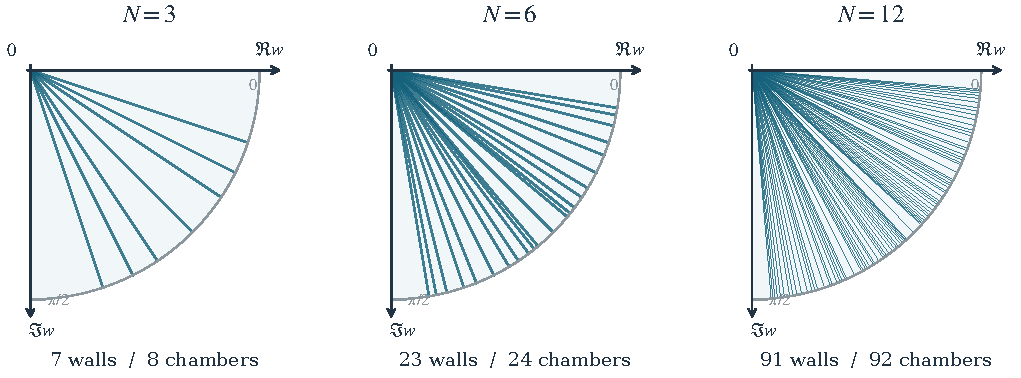
\includegraphics[width=\textwidth]{figures/finite_angular_atlases.pdf}
\caption{Finite rate-ordering atlases for the two actions $1$ and $\ii$.
The degree cutoffs $3,6,12$ have respectively $7,23,91$ interior walls.
The all-orders wall set is dense, while each finite cutoff is explicit.
These lines mark changes of exponential-rate ordering, not Stokes jumps.}
\label{fig:atlas}
\end{figure}

Polynomial or logarithmic amplitudes change the comparison of full
term magnitudes by lower-order contributions. For example a power
factor can shift a simple wall by $O(\log R/R)$. The theorem above
orders \emph{exponential rates}. Uniform control of such moving,
amplitude-sensitive walls is a separate extension discussed below.

\section{The exact two-action convergence domain and its quartic boundary}\label{sec:quartic}

The preceding certificate is uniform over all finite alphabets. It loses
information when complex action vectors partially cancel inside
$\Lambda_{\nn}^{|\nn|-1}$. For the orthogonal pair $1,\ii$ we can retain
that information and determine the full domain of absolute convergence.
The coefficient formula and the saddle method are classical; the exact
calculation below is the model-specific result.

Set $A=|a\e^{-w}|$, $B=|b\e^{-\ii w}|$, and define the absolute
contribution of total degree $N$ by
\begin{equation}\label{eq:DN}
 D_N(A,B)=\sum_{m+n=N}\frac{|m+\ii n|^{N-1}}{m!n!}A^mB^n.
\end{equation}
For $0<p<1$, put
\begin{align}
 r(p)&=\sqrt{p^2+(1-p)^2},\nonumber\\
 H(p)&=-p\log p-(1-p)\log(1-p),\nonumber\\
 \Psi_{A,B}(p)&=1+\log r(p)+H(p)+p\log A+(1-p)\log B,\label{eq:Psi}\\
 \mathcal R(A,B)&=\exp\left(\max_{0\le p\le1}\Psi_{A,B}(p)\right).
 \label{eq:R-variational}
\end{align}
Endpoint values are defined by continuity. The notation $\mathcal R$
denotes a coefficient growth factor, not a radius in the $w$-plane.

\begin{theorem}[Sharp convergence and boundary exponents]\label{thm:exact-domain}
For $A,B>0$, the inverse series \eqref{eq:orthogonal-inverse} converges
absolutely if and only if $\mathcal R(A,B)\le1$. Its maximizing proportion
$p_*$ is unique, lies in $(0,1)$, and satisfies
\begin{equation}\label{eq:pstar}
 \log\frac AB+\log\frac{1-p_*}{p_*}
 +\frac{2p_*-1}{p_*^2+(1-p_*)^2}=0.
\end{equation}
For $A\ne B$,
\begin{equation}\label{eq:gaussian-degree}
 D_N(A,B)\sim\frac{r(p_*)}{\sqrt{2\pi}|2p_*-1|}
 \mathcal R(A,B)^N N^{-3/2}.
\end{equation}
For $A=B=q>0$,
\begin{equation}\label{eq:quartic-degree}
 \mathcal R(q,q)=\e\sqrt2 q,\qquad
 D_N(q,q)\sim C_4(\e\sqrt2 q)^N N^{-5/4},\qquad
 C_4=\frac{3^{1/4}\Gamma(1/4)}{2\sqrt2\pi}.
\end{equation}
Thus the symmetric boundary is exactly $q=1/(\e\sqrt2)$, and absolute
convergence holds on that boundary.
\end{theorem}

\begin{proof}
Differentiation gives
\begin{equation}\label{eq:Phi-second}
 \Psi_{A,B}''(p)=
 -\frac{(2p-1)^2}{p(1-p)\bigl(p^2+(1-p)^2\bigr)^2}.
\end{equation}
It is negative except at $p=1/2$. Hence $\Psi'$ is strictly decreasing;
its endpoint limits are $+\infty$ and $-\infty$. This proves the
existence and uniqueness of the maximizer and \eqref{eq:pstar}.
The maximizer is $1/2$ exactly when $A=B$.

For $p=m/N$ in a compact subinterval of $(0,1)$, uniform Stirling
asymptotics express the corresponding summand of \eqref{eq:DN} as
\begin{equation}\label{eq:saddle-summand}
 \frac{\exp(N\Psi_{A,B}(p))}{2\pi N^2r(p)\sqrt{p(1-p)}}
 \bigl(1+O(N^{-1})\bigr).
\end{equation}
The endpoints are harmless: $\binom Nm\le\exp(NH(p))$ and the lower
Stirling bound for $N!$ bound every summand by
$C N^{-3/2}\exp(N\Psi_{A,B}(p))$, uniformly even at $p=0,1$.
Any closed set separated from $p_*$ has an exponent smaller by a
positive constant and contributes exponentially little.

If $p_*\ne1/2$, put $p=p_*+uN^{-1/2}$. The exponent difference tends to
$\Psi''(p_*)u^2/2$, and the rescaled lattice spacing is $N^{-1/2}$.
A local quadratic upper bound supplies Gaussian domination. The
resulting Riemann sum yields
\[
 D_N\sim\frac{\mathcal R^N N^{-3/2}}
 {\sqrt{2\pi}\,r(p_*)\sqrt{p_*(1-p_*)}\sqrt{-\Psi''(p_*)}}.
\]
Substitution of \eqref{eq:Phi-second} gives \eqref{eq:gaussian-degree}.

If $A=B=q$, write $p=1/2+x$. Direct expansion gives
\begin{equation}\label{eq:quartic-expansion}
 \Psi_{q,q}(1/2+x)=1+\log(\sqrt2 q)
 -\frac{16}{3}x^4+\frac{128}{15}x^6+O(x^8).
\end{equation}
The quadratic term cancels. Set $x=uN^{-1/4}$; the lattice spacing in
$u$ is $N^{-3/4}$ and the prefactor in \eqref{eq:saddle-summand}, without
$N^{-2}$, tends to $\sqrt2/\pi$. A quartic upper bound near zero and
the previous exponential estimate away from zero justify dominated
Riemann-sum convergence. Therefore
\[
 D_N\sim\mathcal R^N N^{-5/4}\frac{\sqrt2}{\pi}
 \int_{\R}\exp(-16u^4/3)\,du.
\]
Substituting $v=(16/3)u^4$ evaluates this integral and gives $C_4$.
For $\mathcal R>1$ the degree sum fails to tend to zero; for
$\mathcal R<1$ it decays geometrically. At $\mathcal R=1$, the
exponents $3/2$ and $5/4$ are both summable. This proves the criterion.
\end{proof}

If one of $A,B$ is zero, the one-action criterion is respectively
$\e B\le1$ or $\e A\le1$. At equal nonzero moduli the exact criterion
improves the general sufficient condition $\e(A+B)<1$ by a factor
$\sqrt2$ in the permitted common modulus.

On $\mathcal R<1$, the series is holomorphic in its two effective
amplitude variables and continues the inverse germ at zero amplitude.
The domain is connected, since scaling both moduli by $t>0$ scales
$\mathcal R$ by $t$. Its inverse equation holds first near zero and
then throughout the domain by analyticity. At $\mathcal R=1$, absolute
convergence gives a continuous radial boundary value still satisfying
that equation. It need not give a holomorphic inverse there.

\subsection{A \texorpdfstring{$4/3$}{4/3}-power law for the convergence boundary}

Write $g=(\log A+\log B)/2$ and $\delta=\log(A/B)$. The optimized
function $\log\mathcal R$ is convex in logarithmic moduli, because it
is a maximum of affine functions of those moduli.

\begin{corollary}[Boundary regularity]\label{cor:boundary-law}
As $\delta\to0$,
\begin{equation}\label{eq:boundary-law}
 \log\mathcal R=1+g+\tfrac12\log2
 +\frac{3^{4/3}}{16}|\delta|^{4/3}
 +\frac3{160}\delta^2+O(|\delta|^{8/3}).
\end{equation}
Consequently the boundary $\mathcal R=1$, expressed as $g(\delta)$,
is $C^1$ but not $C^2$ at zero.
\end{corollary}

\begin{proof}
The local optimization is
$\max_x(\delta x-16x^4/3+128x^6/15+O(x^8))$.
Its maximizer satisfies $x=(3\delta/64)^{1/3}+O(\delta)$, with the
real cube root. More precisely, put
$t=\operatorname{sgn}(\delta)|\delta|^{1/3}$ and $x=ty$. The critical
equation divided by $t^3$ has a nonzero derivative in $y$ at
$t=0$, $y=3^{1/3}/4$. The analytic implicit-function theorem gives
an expansion of $y$ in $t^2$. The leading quartic optimum is
$3^{4/3}|\delta|^{4/3}/16$. The $x^6$ term evaluated at its leading
maximizer contributes $3\delta^2/160$. Displacement of that maximizer
changes the value only at order $|\delta|^{8/3}$, since the leading
part is stationary. This proves \eqref{eq:boundary-law}.
The derivative of the optimized part in $\delta$ equals the unique
maximizing $x$, which behaves as a nonzero multiple of
$\operatorname{sgn}(\delta)|\delta|^{1/3}$. The regularity statement follows.
\end{proof}

This $4/3$ exponent describes the graph of a convergence boundary. It
does not identify that graph with the discriminant of a general cusp
catastrophe.

\subsection{The transition as the action angle varies}

Rotate two unit actions to $\lambda_+=\e^{\ii\beta/2}$,
$\lambda_-=\e^{-\ii\beta/2}$, where $0<\beta<\pi$. Both remain in a
strict cone. For equal effective moduli $q$, replace $r(p)$ by
\begin{equation}\label{eq:rbeta}
 \begin{aligned}
 r_\beta(p)&=|p\lambda_++(1-p)\lambda_-|,\\
 r_\beta(p)^2&=c^2\bigl(1+t^2(2p-1)^2\bigr),
 \qquad c=\cos(\beta/2),\quad t=\tan(\beta/2).
 \end{aligned}
\end{equation}
The degree growth is governed by $\log r_\beta+H$.

\begin{proposition}[Angular saddle transition]\label{prop:angle-transition}
For $0<\beta<\pi/2$, the unique maximizing proportion is $1/2$ and
\begin{equation}\label{eq:subcritical-angle}
 D_N(q,q;\beta)\sim
 \frac{(2\e q\cos(\beta/2))^N}{\sqrt{2\pi\cos\beta}\,N^{3/2}}.
\end{equation}
At $\beta=\pi/2$ the maximum is quartic and
\eqref{eq:quartic-degree} applies. For $\pi/2<\beta<\pi$, exactly
two nondegenerate proportions maximize the exponent. Their distances
from $1/2$ are $y_*/2$, where $y_*\in(0,1)$ uniquely solves
\begin{equation}\label{eq:angle-critical-p}
 \frac{\operatorname{artanh}y_*}{y_*}=
 \frac{t^2}{1+t^2y_*^2}.
\end{equation}
Both contribute ordinary $N^{-3/2}$ terms.
\end{proposition}

\begin{proof}
In the coordinate $y=2p-1$, the derivative of $\log r_\beta+H$ is
$t^2y/(1+t^2y^2)-\operatorname{artanh}y$.
For $y>0$, the quotient $\operatorname{artanh}y/y$ increases strictly
from $1$ to infinity, as its positive power series shows. The right
side of \eqref{eq:angle-critical-p} decreases strictly.
For $t^2\le1$ there is no positive crossing. For $t^2>1$ there is
exactly one, and it is strict; symmetry gives the negative maximizer.
These crossings are nondegenerate. For $\beta<\pi/2$, the second
derivative in $p$ at the center is $4(t^2-1)<0$. Substituting it into
the lattice Gaussian calculation gives
$1/\sqrt{2\pi\cos\beta}$. The critical quartic case was already proved.
\end{proof}

\subsection{A uniform critical crossover and its first correction}\label{sec:crossover}

The two sides of the angular transition fit into one uniform theorem.
For $q>0$ and real $\tau,\eta$, set
\begin{equation}\label{eq:double-scaling}
 \beta_N=\frac\pi2+\frac\tau{\sqrt N},\quad
 \delta_N=\frac\eta{N^{3/4}},\quad
 A_N=q\e^{\delta_N/2},\quad B_N=q\e^{-\delta_N/2}.
\end{equation}
Here $D_N(A,B;\beta)$ replaces $|m+\ii n|$ in \eqref{eq:DN} by
$|m\lambda_++n\lambda_-|$, with $\lambda_\pm=\e^{\pm\ii\beta/2}$.

\begin{theorem}[Uniform quartic profile]\label{thm:quartic-crossover}
Define
\begin{align}
 \mathcal P(\tau,\eta)&=\frac{\sqrt2}{\pi}\int_{\R}
 \exp\left(4\tau u^2+\eta u-\frac{16}{3}u^4\right)\,du,
 \label{eq:quartic-profile}\\
 P_\tau(u)&=\frac\tau2+4\tau^2u^2-16\tau u^4+\frac{128}{15}u^6,
 \label{eq:profile-poly}\\
 \mathcal P_1(\tau,\eta)&=\frac{\sqrt2}{\pi}\int_{\R}P_\tau(u)
 \exp\left(4\tau u^2+\eta u-\frac{16}{3}u^4\right)\,du.
 \label{eq:quartic-profile-one}
\end{align}
Uniformly for $(\tau,\eta)$ in any compact subset of $\R^2$,
\begin{equation}\label{eq:quartic-crossover}
 \frac{N^{5/4}D_N(A_N,B_N;\beta_N)}
 {[2\e q\cos(\beta_N/2)]^N}
 =\mathcal P(\tau,\eta)+N^{-1/2}\mathcal P_1(\tau,\eta)+O(N^{-1}).
\end{equation}
The factor $q$ cancels exactly from the normalized expression.
\end{theorem}

\begin{proof}
Put $p=1/2+x$, $c_N=\cos(\beta_N/2)$,
$t_N=\tan^2(\beta_N/2)$ and
\[
 \Xi_N(x)=H(1/2+x)-\log2+\tfrac12\log(1+4t_Nx^2)+\delta_Nx.
\]
After removing the central exponential factor, uniform Stirling
expansion on a fixed central interval gives each summand as
\begin{equation}\label{eq:crossover-summand}
 \frac{1+O(N^{-1})}{2\pi N^2}
 \frac{\exp(N\Xi_N(x))}
 {c_N\sqrt{1+4t_Nx^2}\sqrt{1/4-x^2}}.
\end{equation}
The entropy inequality
$H(1/2+x)\le\log2-2x^2-4x^4/3$, valid also by continuity at the
endpoints, and $\log(1+y)\le y$ give
\[
 \Xi_N(x)\le2(t_N-1)x^2-\tfrac43x^4+\delta_Nx.
\]
Since $t_N-1=O(N^{-1/2})$, the coordinate $u=N^{1/4}x$ gives a
uniform bound
\begin{equation}\label{eq:quartic-domination}
 N\Xi_N(uN^{-1/4})\le C u^2-\tfrac43u^4+E|u|.
\end{equation}
Outside any fixed central interval the entropy upper bound for
binomial coefficients makes the normalized sum exponentially small.
This handles $p=0,1$ without an invalid endpoint Stirling approximation.

Taylor expansion gives
$t_N=1+2\tau N^{-1/2}+2\tau^2N^{-1}+O(N^{-3/2})$ and
\begin{align*}
 N\Xi_N(uN^{-1/4})
 ={}&4\tau u^2+\eta u-16u^4/3\\
 &+N^{-1/2}\bigl(4\tau^2u^2-16\tau u^4+128u^6/15\bigr)\\
 &+O\bigl(N^{-1}(u^2+u^4+u^6+u^8)\bigr).
\end{align*}
The smooth prefactor has a further cancellation:
\begin{align*}
 \frac{1}{c_N\sqrt{1+4t_Nx^2}\sqrt{1/4-x^2}}
 &=\frac{2}{c_N}\bigl[(1+4t_Nx^2)(1-4x^2)\bigr]^{-1/2}\\
 &=2\sqrt2\left[1+\frac{\tau}{2\sqrt N}
 +O\bigl(N^{-1}(1+u^2+u^4)\bigr)\right].
\end{align*}
There is no $u^2N^{-1/2}$ contribution from this prefactor.

Choose the fixed central interval sufficiently small. Taylor's theorem
for the real exponential, together with \eqref{eq:quartic-domination},
then bounds the difference between the scaled summands and their first
two displayed terms by
\[
 h_N N^{-1}Q(u)\exp(C_1u^2-c_1u^4+E|u|),
 \qquad h_N=N^{-3/4},\quad c_1>0,
\]
where $Q$ is a fixed polynomial. To see why the bound is uniform on
the whole central interval, note that $N^{-1/2}u^6\le\epsilon^2u^4$
when $|x|\le\epsilon$; choosing $\epsilon$ small preserves negative
quartic domination. The higher remainders are treated in the same way.

The $u$-grid has spacing $h_N$, independently of its parity-dependent
shift. The functions $\exp(4\tau u^2+\eta u-16u^4/3)$ and its product
with $P_\tau$, including their first two derivatives, have uniformly
bounded integrals of absolute value on compact parameter sets. The
midpoint-cell estimate
\[
 \left|h\sum_{k\in\Z}f(a+kh)-\int_\R f(u)\,du\right|
 \le C h^2\norm{f''}_{L^1}
\]
follows by integrating Taylor's formula on each centered cell. It
makes the lattice error $O(N^{-3/2})$. The integrable remainder above
sums to $O(N^{-1})$. Multiplying the central prefactor by the mesh
factor proves \eqref{eq:quartic-crossover}.
\end{proof}

At the critical point $\mathcal P(0,0)=C_4$. The profile extends to
an entire function of its two complex parameters, is even in $\eta$,
and satisfies
\begin{equation}\label{eq:profile-pdes}
 \partial_\tau\mathcal P=4\partial_\eta^2\mathcal P,
 \qquad
 \frac{64}{3}\partial_\eta^3\mathcal P
 -8\tau\partial_\eta\mathcal P-\eta\mathcal P=0.
\end{equation}
Both identities follow by differentiation under the quartically
dominated integral and integration by parts. They provide a convenient
way to generate its moment corrections. The theorem identifies
$N^{-1/2}$ as the angle scale and $N^{-3/4}$ as the amplitude-imbalance
scale; it is more informative than separate limiting exponents.

\subsection{A cubic critical point reached by the selected branch}

Take
\begin{equation}\label{eq:cubic-example}
 a=b=\frac{1-\ii}{2},\qquad
 F(z)=z+a\e^{-z}+b\e^{-\ii z},\qquad w_0=1-\ii.
\end{equation}
Direct calculation gives
\begin{equation}\label{eq:cubic-derivatives}
 F(0)=w_0,\quad F'(0)=F''(0)=0,\quad F'''(0)=\ii.
\end{equation}
Both effective moduli at $w_0$ are $1/(\e\sqrt2)$, so this critical
value lies exactly on the symmetric absolute-convergence boundary.

To identify the branch, scale both amplitudes by $t\in[0,1]$ and set
$z=(1-\ii)v$. The equation $F_t(z)=w_0$ becomes
\[
 v+t\e^{-v}\cos v=1,\qquad
 t(v)=\frac{(1-v)\e^v}{\cos v},\quad 0\le v\le1.
\]
It maps $v=1$ to $t=0$ and $v=0$ to $t=1$ and is strictly decreasing
between them, because $(\log t)'=\tan v-v/(1-v)<0$.
For the inequality, $v\cos v-(1-v)\sin v$ vanishes at zero and has
positive derivative $(1-v)\sin v+v\cos v$ on $(0,1)$.
Along this path,
$F_t'((1-\ii)v)=v-(1-v)\tan v>0$ for $0<v<1$,
so the inverse branch stays simple before the endpoint.
Thus the branch selected at zero amplitude reaches $z=0$ at $t=1$.
Moreover $t(v)=1-v^3/3+O(v^4)$.

For the fixed function $F$, its three local inverse branches have
\begin{equation}\label{eq:cubic-root}
 z=\left(\frac{6(w-w_0)}{\ii}\right)^{1/3}
 +O((w-w_0)^{2/3}).
\end{equation}
The exponent $1/3$ is an inverse ramification exponent. The exponent
$5/4$ concerns sums of absolute values of bivariate coefficients at
one degree. Complex phase cancellations distinguish the quantities;
one exponent should not be read off from the other.

\begin{figure}[tbp]
\centering
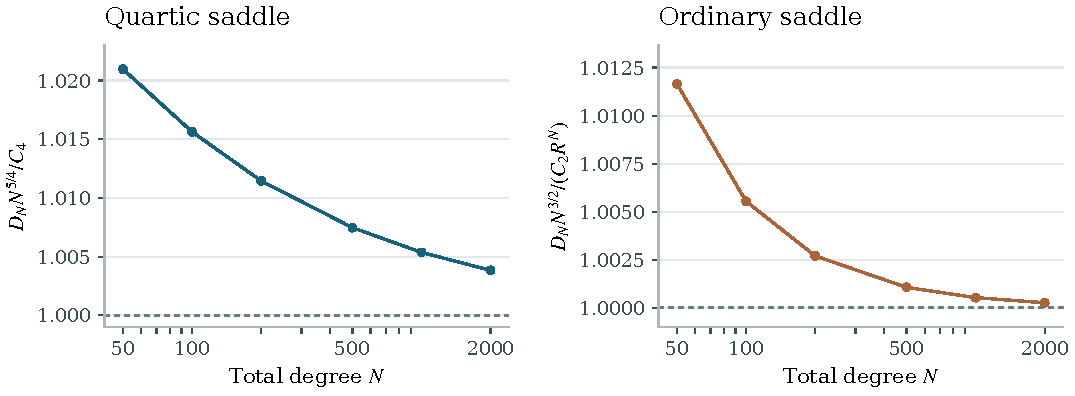
\includegraphics[width=0.96\textwidth]{figures/quartic_saddle_scaling.pdf}
\caption{Checks of the quartic and Gaussian degree laws. The balanced
case is normalized by $C_4N^{-5/4}$ at its convergence boundary. The
unbalanced case uses its own growth factor and Gaussian prefactor.
The proof rests on the localized lattice-saddle argument, not the
finite numerical comparisons.}\label{fig:quartic}
\end{figure}

\section{A sharp Borel majorant and inverse-domain certificate}\label{sec:borel}

The inverse Borel formula and the exponential bound
$M\e^{(\tau+2\sqrt M)|\zeta|}$ already appear in the repository's
\emph{Negative-Ray Summation of Exponential Feedback}, Lemma
\texttt{lem:fineinverse} \cite{repo-negative}. The refinement here is
the exact Bessel majorant, its pointwise optimality, and the matching
source and target half-plane bounds. The next section applies them
uniformly to sine-period families.

Let $K$ be holomorphic near zero and on a star-shaped open sector of
the Borel plane. Assume, on the rays being used, that
\begin{equation}\label{eq:K-bound}
 |K(\zeta)|\le M\e^{\tau|\zeta|},\qquad M>0,\quad\tau\ge0.
\end{equation}
Let $\widetilde h=\B^{-1}K$ and let
$\widetilde G=z+\widetilde v$ be the formal inverse of
$z+\varepsilon\widetilde h(z)$.

\begin{theorem}[Optimal Bessel majorant]\label{thm:bessel}
Set $a=|\varepsilon|M$. The inverse Borel transform is
\begin{equation}\label{eq:inverse-borel}
 \widehat v(\zeta)=
 -\sum_{n\ge1}\frac{\varepsilon^n}{n!}\zeta^{n-1}K^{*n}(\zeta).
\end{equation}
It converges normally on the same star sector and satisfies, for
$r=|\zeta|$,
\begin{equation}\label{eq:bessel-bound}
 |\widehat v(\zeta)|\le
 a\e^{\tau r}\frac{I_1(2\sqrt a\,r)}{\sqrt a\,r}
 \le a\e^{(\tau+2\sqrt a)r}.
\end{equation}
The quotient is defined as $1$ at $a r^2=0$. Both the pointwise
majorant and its universal exponential-type bound are sharp.
\end{theorem}

\begin{proof}
Formal Lagrange inversion gives
$\widetilde v=\sum_{n\ge1}(-\varepsilon)^n
\D^{n-1}(\widetilde h^n)/n!$. Its $n$th term has order at least
$z^{-(2n-1)}$, so substitution of $\varepsilon$ is formally legitimate
coefficient by coefficient. The Borel rules in
\eqref{eq:borel-convention} give \eqref{eq:inverse-borel}.

The $n$-fold straight-segment convolution is an integral over a simplex
of volume $r^{n-1}/(n-1)!$. The lengths of its arguments sum to $r$.
Consequently
\begin{equation}\label{eq:simplex-bound}
 |K^{*n}(\zeta)|\le
 M^n\e^{\tau r}\frac{r^{n-1}}{(n-1)!}.
\end{equation}
Summing gives
\[
 |\widehat v(\zeta)|\le\e^{\tau r}
 \sum_{n\ge1}\frac{a^n r^{2n-2}}{n!(n-1)!}
 =a\e^{\tau r}\frac{I_1(2\sqrt a r)}{\sqrt a r},
\]
where the equality can also be taken as the defining power series of
this Bessel quotient. Its normal convergence justifies the analytic
Borel formula. For $t\ge0$,
\[
 \frac{I_1(2t)}t=\sum_{k\ge0}\frac{t^{2k}}{k!(k+1)!}
 \le\cosh(2t)\le\e^{2t};
\]
the first inequality uses
$(2k)!/(k!(k+1)!)\le4^k$.

For sharpness choose $K(\zeta)=M\e^{\tau\zeta}$ and real
$\varepsilon>0$. Then
$K^{*n}=M^n\e^{\tau\zeta}\zeta^{n-1}/(n-1)!$.
All terms of \eqref{eq:inverse-borel} have the same sign on the
positive ray, so equality holds in the first bound.
The integral identity
\[
 \frac{I_1(2t)}t=\frac2\pi\int_{-1}^{1}
 \e^{2tu}\sqrt{1-u^2}\,du
\]
follows by expanding the exponential and evaluating beta integrals.
It shows that its logarithmic growth rate is $2$: the upper bound
was proved, and restriction to $u\in[1-\delta,1-\delta/2]$ gives
every lower exponential rate $2(1-\delta)$. Thus the attained rate
in \eqref{eq:bessel-bound} is $\tau+2\sqrt a$.
\end{proof}

\begin{theorem}[Sharp half-plane inversion certificate]\label{thm:halfplane}
Fix a Borel direction $\theta$ satisfying \eqref{eq:K-bound}, and set
$h_\theta=\Lap_\theta K$, $F_\theta=z+\varepsilon h_\theta$.
Then $F_\theta$ is univalent on
\begin{equation}\label{eq:source-halfplane}
 \Rea(\e^{\ii\theta}z)>\tau+\sqrt a.
\end{equation}
Its image contains the target half-plane
\begin{equation}\label{eq:target-halfplane}
 \Rea(\e^{\ii\theta}w)>\tau+2\sqrt a.
\end{equation}
There the inverse is $G_\theta(w)=w+\Lap_\theta\widehat v(w)$ and,
with $q=\Rea(\e^{\ii\theta}w)-\tau$,
\begin{equation}\label{eq:catalan-displacement}
 |G_\theta(w)-w|\le\frac{q-\sqrt{q^2-4a}}2.
\end{equation}
The source and target thresholds are optimal as universal constants
under \eqref{eq:K-bound}.
\end{theorem}

\begin{proof}
Direct Laplace estimates give
\[
 |\varepsilon h_\theta(z)|\le\frac{a}{q_z},\qquad
 |\varepsilon h_\theta'(z)|\le\frac{a}{q_z^2},
 \quad q_z=\Rea(\e^{\ii\theta}z)-\tau>0.
\]
On the convex half-plane \eqref{eq:source-halfplane}, integrate the
derivative of the perturbation along each line segment. Its modulus
is strictly below one on that segment, proving injectivity.

If $q>2\sqrt a$, use the disk centered at $w$ of radius $q/2$.
On it the perturbation has norm at most $2a/q<q/2$.
Rouch\'e gives a unique root with displacement $d<q/2$, and
the root equation gives $d\le a/(q-d)$.
Since $d(q-d)$ increases on $[0,q/2]$, this implies
\eqref{eq:catalan-displacement}. Its image lies in the source
half-plane, because $q-d\ge(q+\sqrt{q^2-4a})/2>\sqrt a$.

Termwise Laplace integration of \eqref{eq:inverse-borel} is justified
by the Bessel majorant. Its positive integral is exactly
\begin{equation}\label{eq:catalan-laplace}
 \sum_{n\ge1}\frac{(2n-2)!}{n!(n-1)!}\frac{a^n}{q^{2n-1}}
 =\frac{q-\sqrt{q^2-4a}}2.
\end{equation}
The coefficients are Catalan numbers. The summed function agrees
with the analytic Lagrange inverse for $q$ sufficiently large and
hence, by analyticity and the preceding range inclusion, throughout
\eqref{eq:target-halfplane}.

For $K=M\e^{\tau\zeta}$, $\theta=0$, $\varepsilon>0$, one has
$F(z)=z+a/(z-\tau)$ and
\begin{equation}\label{eq:sharp-quadratic}
 G(w)=\frac{w+\tau+\sqrt{(w-\tau)^2-4a}}2,
\end{equation}
with the square root selected at infinity. The positive critical
source point is $\tau+\sqrt a$ and its value is $\tau+2\sqrt a$.
Equality also holds in \eqref{eq:catalan-displacement} on the
positive real target ray. Neither universal threshold can be lowered.
\end{proof}

The sign distinction is useful: $\widehat v$ is negative on the
positive ray in the sharp model. The positive expression in
\eqref{eq:catalan-laplace} is the majorant for $|G-w|$, not the
signed displacement $G-w$.

\section{A sine-kernel family: uniform bounds and filtered continuation}\label{sec:sine}

The next application separates two questions that should not be conflated:
uniform estimates on straight nonreal summation rays, and continuation along
more general paths that may reach other sheets. The first follows from an
elementary estimate; the second uses a published nonlinear continuation theorem.

\subsection{Uniform inversion away from real Borel directions}

For $\alpha>0$ consider the meromorphic kernel
\begin{equation}\label{eq:sine-kernel}
 K_\alpha(\zeta)=
 \frac{\zeta^2}{\sin(\pi\zeta)\sin(\pi\alpha\zeta)}.
\end{equation}
The origin is removable, with $K_\alpha(0)=1/(\pi^2\alpha)$.
Its possible poles belong to
\[
 \Sigma_\alpha=(\Z\cup\alpha^{-1}\Z)\setminus\{0\}.
\]
At rational $\alpha$, nonzero poles from the two lattices can coincide.
At irrational $\alpha$, distinct poles can approach one another arbitrarily
closely at large distance. Splitting the kernel into individual residues is
therefore poorly suited to estimates uniform in $\alpha$.

\begin{theorem}[Period-uniform sectorial inverse bounds]\label{thm:sine-uniform}
Fix $0<\alpha_0\le\alpha_1<\infty$ and $0<\eta\le\pi/2$.
For every $\alpha\in[\alpha_0,\alpha_1]$ and every ray angle $\theta$
with $|\sin\theta|\ge\sin\eta$,
\begin{equation}\label{eq:sine-uniform}
 |K_\alpha(r\e^{\ii\theta})|
 \le M_\eta:=\frac1{\pi^2\alpha_0\sin^2\eta},
 \qquad r\ge0.
\end{equation}
Let $h_{\alpha,\theta}=\Lap_\theta K_\alpha$ and
$a_\eta=|\varepsilon|M_\eta$.
The map $F_{\alpha,\theta}=z+\varepsilon h_{\alpha,\theta}$ is
univalent on
\[
 \Rea(\e^{\ii\theta}z)>\sqrt{a_\eta},
\]
and its image contains
\[
 \Rea(\e^{\ii\theta}w)>2\sqrt{a_\eta}.
\]
On the latter half-plane, its inverse satisfies
\[
 |G_{\alpha,\theta}(w)-w|
 \le \frac{q-\sqrt{q^2-4a_\eta}}2,
 \qquad q=\Rea(\e^{\ii\theta}w),
\]
and the inverse Borel transform has the uniform bound
\[
 |\widehat v_\alpha(r\e^{\ii\theta})|
 \le a_\eta\frac{I_1(2\sqrt{a_\eta}\,r)}
                  {\sqrt{a_\eta}\,r}
 \le a_\eta\e^{2\sqrt{a_\eta}\,r}.
\]
These statements hold uniformly through rational values of $\alpha$.
\end{theorem}

\begin{proof}
The elementary identity
\[
 |\sin(x+\ii y)|^2=\sin^2x+\sinh^2y
\]
gives $|\sin(x+\ii y)|\ge\sinh|y|\ge|y|$.
Applying it to the two denominator factors yields, for $r>0$,
\[
 |K_\alpha(r\e^{\ii\theta})|
 \le \frac{r^2}
 {\pi r|\sin\theta|\,\pi\alpha r|\sin\theta|}
 \le M_\eta.
\]
Continuity gives the same bound at zero. The preceding Borel and
half-plane theorems now apply with $\tau=0$.

For completeness, continuity in $\alpha$ follows directly from the
unsplit kernel. On every compact part of an off-axis ray, the removable
value at zero and the nonvanishing denominators give continuous
dependence on $\alpha$. The uniform bound controls the Laplace tail
on every strictly smaller target half-plane. The Bessel majorant
also permits termwise passage to the limit in the inverse Borel
series. Coinciding real poles create no exceptional case.
\end{proof}

This theorem is a uniformity statement, not an assertion that $M_\eta$
is optimal for this particular family. Optimality in \cref{thm:halfplane}
concerns the full class of kernels with a given bound.
Also, $M_\eta$ diverges as $\eta\downarrow0$.
The argument gives neither a uniform approach to a real Stokes direction
nor uniform bounds on arbitrary continuation sheets.

As a normalization check, the formal Laplace series begins
\[
 h_\alpha(z)=\frac1{\pi^2\alpha z}
       +\frac{1+\alpha^2}{3\alpha z^3}+O(z^{-5}).
\]
These are coefficients of the asymptotic formal series; the actual
function is specified by the chosen summation direction.

\subsection{The continuation-cost set}

Suppose now that $\alpha$ is irrational, and write
$\ell_1=1$, $\ell_2=\alpha^{-1}$.
Define a family of finite sets by
\begin{equation}\label{eq:filtered-sine}
 \sincost_L=
 \left\{\omega_1+\cdots+\omega_n:
 \begin{array}{l}
 n\ge1,\quad \omega_j\in\Sigma_\alpha,\\
 |\omega_1|+\cdots+|\omega_n|\le L
 \end{array}\right\}.
\end{equation}
The budget records the sum of the costs of the primitive pieces.
It is not the modulus of their final sum.

\begin{proposition}[Explicit saturated cost]\label{prop:cost}
For irrational $\alpha$,
\begin{align}
 \sincost_L
 ={}&\{m\ell_1+n\ell_2:
 (m,n)\in\Z^2\setminus\{(0,0)\},\nonumber\\
 &\hspace{2em}|m|\ell_1+|n|\ell_2\le L\}\nonumber\\
 &{}\cup
 \begin{cases}
 \{0\},&L\ge2\min(\ell_1,\ell_2),\\
 \varnothing,&L<2\min(\ell_1,\ell_2).
 \end{cases}
 \label{eq:cost-explicit}
\end{align}
Every $\sincost_L$ is finite, whereas
$\bigcup_{L\ge0}\sincost_L=\ell_1\Z+\ell_2\Z$ is dense in $\R$.
The family is empty for sufficiently small $L$, is increasing and
right-continuous in $L$, and satisfies
\[
 \sincost_{L_1}+\sincost_{L_2}\subseteq\sincost_{L_1+L_2}.
\]
\end{proposition}

\begin{proof}
Irrationality makes the integer representation
$m\ell_1+n\ell_2$ unique. In any primitive word representing this
point, separate the two lattices and apply the triangle inequality
to each integer sum. Its cost is at least
$|m|\ell_1+|n|\ell_2$. If $(m,n)\ne(0,0)$, this lower bound is attained
by using the nonzero terms $m\ell_1$ and $n\ell_2$, omitting a zero term.
A nonempty word representing zero must have zero total integer
coefficient in each lattice. It must therefore contain a cancellation
within at least one lattice. Its cost is at least
$2\min(\ell_1,\ell_2)$, attained by the shortest opposite pair.

The explicit integer bounds prove finiteness at each budget and
right-continuity. Concatenating words proves the additive inclusion.
To see density, irrationality and the pigeonhole principle produce
nonzero elements of $\ell_1\Z+\ell_2\Z$ of arbitrarily small modulus.
Their integer multiples approximate any real number to within
half that modulus.
\end{proof}

The delayed zero in \eqref{eq:cost-explicit} is essential.
The original Borel germ is regular at zero. The empty word must not
place zero in the forbidden set at cost zero. A possible singularity
over zero reached after a nontrivial continuation history is a
different object.

\begin{figure}[htbp]
\centering
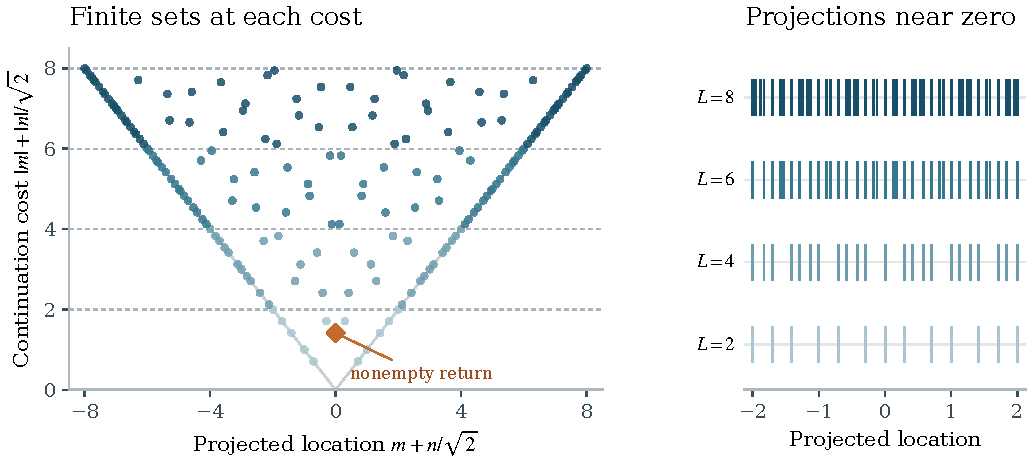
\includegraphics[width=0.96\textwidth]{figures/cost_filtered_locations.pdf}
\caption{Potential Borel locations for $\alpha=\sqrt2$, filtered by
the cost $|m|+|n|/\sqrt2$. The projection is globally dense, while
every fixed budget contains finitely many locations. Zero appears
only after the nonempty return cost $\sqrt2$. The figure displays
possible locations; it does not assert that each is singular.}
\label{fig:cost}
\end{figure}

\subsection{An application of filtered implicit-function theory}\label{sec:filtered}

A discrete filtered set is, in the terminology of Kamimoto and
Sauzin \cite[Definitions 2.1--2.8]{kamimoto-sauzin}, a family of
finite subsets of $\C$ that increases with a length budget and is
empty at sufficiently small budget, with the relevant upper closure
used in defining admissible paths. For the right-continuous family
above, a piecewise smooth path $\gamma$ starting at zero is allowed
when
\[
 \gamma(t)\notin\sincost_{\operatorname{length}(\gamma|_{[0,t]})}
 \quad\text{for all }t.
\]
The condition is imposed on the pair consisting of accumulated length
and current position, not merely on the image of the path.

\begin{theorem}[Filtered continuation of the inverse]\label{thm:filtered}
Let $h_\alpha$ be the formal inverse-power series with
$\B h_\alpha=K_\alpha$, and let
$G_\alpha(w)=w+v_\alpha(w)$ be the formal compositional inverse of
$z+\varepsilon h_\alpha(z)$.
For irrational $\alpha>0$, $\B v_\alpha$ admits analytic continuation
along every $\sincost$-allowed path, with $\sincost$ given by
\eqref{eq:filtered-sine}--\eqref{eq:cost-explicit}.
For rational $\alpha>0$, the same conclusion holds with the
word-cost definition \eqref{eq:filtered-sine}, with coincident
locations identified.
\end{theorem}

\begin{proof}
This is an application of the Kamimoto--Sauzin implicit-function
theorem \cite[Theorem 5.3]{kamimoto-sauzin}; we verify its relevant
inputs rather than reprove its continuation estimates.

Start with the filtered set
$\Omega_L=\{\omega\in\Sigma_\alpha:|\omega|\le L\}$.
It is finite at fixed $L$. The meromorphic function $K_\alpha$ is
holomorphic along every $\Omega$-allowed path, because a path that
reaches a pole $\omega$ has length at least $|\omega|$.
Multiplication of $K_\alpha$ by a polynomial creates no new
singular locations. Thus every coefficient in
\begin{equation}\label{eq:implicit-filtered}
 \mathcal F(z,u)=u+
 \varepsilon\sum_{k\ge0}\frac{h_\alpha^{(k)}(z)}{k!}\,u^k
\end{equation}
has the required filtered continuation. For the compact sets
$K_\Omega^{\delta,L}$ of \cite[Notation 3.15]{kamimoto-sauzin},
on the continuation surface with projection $p_\Omega$, put
\[
 M_{\delta,L}=
 \sup_{\xi\in K_\Omega^{\delta,L}}
 |K_\alpha(p_\Omega(\xi))|<\infty.
\]
Every such $\xi$ is reached by a path of length at most $L$, so
$|p_\Omega(\xi)|\le L$. Writing
$\mathcal F(z,u)=\sum_{k\ge0}\mathcal F_k(z)u^k$, the seminorms
of \cite[Definition 3.16]{kamimoto-sauzin} satisfy
\[
 \norm{\mathcal F_k}_\Omega^{\delta,L}
 \le \mathbf 1_{\{k=1\}}
       +|\varepsilon|M_{\delta,L}\frac{L^k}{k!}
 \le C_{\delta,L}^{\,k+1}
 \qquad(k\ge0)
\]
for a suitable $C_{\delta,L}\ge1$.
This verifies precisely the coefficient-growth condition in
\cite[Definition 5.1]{kamimoto-sauzin}, including the scalar $u$ term.
The constants here can depend on the fixed $\alpha$ and
$\varepsilon$; no uniformity on later sheets is inferred.

The constant term at $z=\infty$ of $\mathcal F$ is $u$, so its value
at $u=0$ is zero and its $u$ derivative there is one.
The unique formal implicit solution therefore exists, and its
Borel transform is continuable with respect to the saturation
$\Omega^{*\infty}$. The filtered convolution operation adds the
primitive costs; its saturation is exactly the nonempty-word set
\eqref{eq:filtered-sine}. This proves the claim.
\end{proof}

No step of this theorem proves that every element of $\sincost_L$
is an actual singularity. The theorem gives a controlled continuation
surface and an upper bound on possible obstructions.
The same distinction appears in Kamimoto and Sauzin's discussion of
dense projected singular sets \cite[Remark 2.17]{kamimoto-sauzin}.
It would be incorrect to infer a natural boundary from density of
the unfiltered projection alone.

The two results in this section complement each other.
\Cref{thm:sine-uniform} supplies explicit constants, uniform in
$\alpha$, on nonreal straight rays.
\Cref{thm:filtered} supplies a broader qualitative continuation
statement for a fixed parameter.
Uniform bounds on later sheets, especially while real poles coalesce,
remain an additional problem.

\section{Finite Stokes transport, logarithmic cores, and the limits of generality}
\label{sec:transport}

\subsection{The exact transition identity}

The inverse of a sectorial jump is nonlinear.
This fact is already developed in the repository's nonlinear Stokes
report \cite{repo-stokes} and in the general resurgent calculus
\cite{sauzin-notes}. It fits naturally with the exact-core theorem.

Let $F_-$ and $F_+$ be two holomorphic realizations with compatible
inverse branches $G_-$ and $G_+$, and set $J=F_+-F_-$ on their common
source domain. On a target domain where the compositions are defined,
\begin{equation}\label{eq:finite-transition}
 T=F_+\circ G_-=\id+J\circ G_-,
 \qquad
 G_+=G_-\circ T^{-1}.
\end{equation}
If $J\circ G_-$ is small in the disk norm of \cref{thm:weighted},
then
\begin{equation}\label{eq:finite-stokes-series}
 G_+-G_-=
 \sum_{n\ge1}\frac{(-1)^n}{n!}
 \D^{n-1}\!\left[G_-'\,(J\circ G_-)^n\right].
\end{equation}
In particular, the first variation is
$-G_-'\,J\circ G_-$, and the higher variations generate all mixed
jump actions.

The proof of \eqref{eq:finite-transition} is composition:
$F_+\circ G_-=T$ implies
$F_+\circ G_-\circ T^{-1}=\id$ on the chosen branch.
Equation \eqref{eq:finite-stokes-series} is then
\cref{thm:weighted} with exact core $G_-$.
If several realizations are indexed by $\alpha,\beta,\gamma$, their
target transition maps satisfy
\[
 T_{\gamma\beta}\circ T_{\beta\alpha}=T_{\gamma\alpha},
 \qquad T_{\beta\alpha}=F_\beta\circ G_\alpha,
\]
whenever the same intermediate inverse branch is used and all
compositions are defined.
This is an analytic transition identity. The dense sorting walls
in \cref{sec:atlas} are not, by themselves, such jumps.

\subsection{A logarithmic core and complex powers}

Consider, on a fixed logarithm branch,
\begin{equation}\label{eq:log-model}
 F(z)=z+\rho\log z+b\e^{-\lambda z}.
\end{equation}
Let $G_0$ be a chosen holomorphic inverse of $z+\rho\log z$,
away from points where $G_0+\rho=0$. Implicit differentiation gives
\begin{align}
 G_0'&=\frac{G_0}{G_0+\rho},&
 G_0''&=\frac{\rho G_0}{(G_0+\rho)^3},&
 G_0'''&=\frac{\rho G_0(\rho-2G_0)}{(G_0+\rho)^5}.
 \label{eq:log-core-derivatives}
\end{align}
With $H=b\e^{-\lambda G_0}$, the exact-core expansion begins
\begin{align}
 G={}&G_0-bG_0'\e^{-\lambda G_0}\nonumber\\
 &+\frac{b^2}{2}
       \left(G_0''-2\lambda(G_0')^2\right)
       \e^{-2\lambda G_0}\nonumber\\
 &-\frac{b^3}{6}
       \left(G_0'''-9\lambda G_0'G_0''
                    +9\lambda^2(G_0')^3\right)
       \e^{-3\lambda G_0}+\cdots .
 \label{eq:log-expansion}
\end{align}
This is convergent whenever the disk smallness hypothesis holds,
and otherwise is a formal amplitude expansion under the appropriate
formal interpretation.

On an admissible asymptotic branch,
\[
 G_0(w)=w-\rho\log w+O(\log w/w).
\]
Consequently,
\begin{equation}\label{eq:complex-power-core}
 \e^{-\lambda G_0(w)}
 =\e^{-\lambda w}w^{\rho\lambda}
       \left(1+O(\log w/w)\right),
\end{equation}
with the complex power defined by that same logarithm branch.
The exponential action remains $\lambda$, but the coefficient
alphabet acquires complex powers and logarithms.
This example explains why preservation of the additive action
semigroup is a weaker assertion than preservation of a prescribed
full transseries alphabet.

The formulas also show where the regular core chart fails:
$G_0+\rho=0$ makes the displayed derivatives singular.
A Puiseux or another critical inverse chart must replace regular
Lagrange inversion there. The repository already treats several
real positive-action critical regimes \cite{repo-moving,repo-critical};
\cref{sec:quartic} exhibits a genuinely complex cubic example.

\subsection{What general transseries require beyond this article}

The weighted theorem applies to arbitrary holomorphic phases
$\Phi_j$, including nonlinear phases, as soon as the stated disk
norms and coefficient controls are proved.
For example, perturbations built from $\e^{-z^2}$ or
$\e^{-\e^z}$ can be handled locally on suitable domains.
The finite linear-action cone theorem does not automatically
establish those domain estimates: a small phase on one ray can
grow rapidly in a disk or in a neighboring direction.

Likewise, a formal inverse in a degree completion does not by itself
choose an analytic realization. Distinct holomorphic functions may
have the same power-log asymptotic expansion and differ by an
exponentially small term. Their inverses need not agree.
A summation prescription, an exact analytic core, or another branch
normalization is therefore part of a meaningful analytic inversion
statement.

Finally, local or sectorial inverse closure does not imply one
single-valued inverse on the entire complex plane.
Already $F(z)=z+\e^{-z}$ has critical points $2\pi\ii k$ and
critical values $1+2\pi\ii k$, $k\in\Z$.
Any global continuation theory has to keep track of inverse sheets
and their monodromy.
Unrestricted complex transseries encompass ordered algebraic,
sectorial analytic, multisummable, resurgent, and higher-level
questions with different hypotheses.
The results here give compatible pieces of that theory rather
than identify these categories.

\section{Further research questions and a proposed programme}\label{sec:questions}

The questions below distinguish extensions that have a clear finite
model from problems requiring a broader analytic category.
They are proposed problems, not claims of established open status
throughout the literature. Their relationship to the inspected
repository is described in \cref{app:provenance}.

\subsection{Exact convergence and critical asymptotics}

\begin{question}[More than two complex actions]\label{q:many-actions}
For $F(z)=z+\sum_{j=1}^s a_j\e^{-\lambda_jz}$, determine the full
absolute-convergence domain of its labelled inverse expansion.
The natural variational quantity on the simplex is
\[
 \Psi(\mathbf p)
 =1+\log\left|\sum_jp_j\lambda_j\right|
    -\sum_jp_j\log p_j+\sum_jp_j\log A_j,
 \qquad A_j=|a_j\e^{-\lambda_jw}|.
\]
Which geometric hypotheses make the maximizer unique?
Which degeneracies are possible, and which boundary degree laws are
summable? A complete result should treat faces of the simplex,
zeros of the action barycenter, and exact action collisions.
\end{question}

The two-action proof suggests a useful first target: three actions
in a strict cone, with an interior maximizer and a Hessian that is
negative definite except on one controlled degeneracy locus.
Ordinary interior saddles are expected to retain the degree exponent
$-3/2$ after the dimensional factors cancel. A proof should specify
the hypotheses under which that cancellation remains uniform.

\begin{question}[Criticality of the majorant versus the actual inverse]
Classify the relation between degeneracies of the absolute degree
sum and ramification of the actual complex inverse.
The orthogonal example has a quartic saddle in the absolute sum and
a cubic critical point for a suitable phase choice.
When does such a correspondence hold, and when does oscillatory
cancellation separate the two phenomena?
\end{question}

A useful answer would distinguish three boundaries: the domain of
absolute convergence of the labelled multivariate series, the
domain of its analytic continuation, and the critical-value set
of the selected inverse sheet. These sets need not coincide.
Generalized Lambert inverses and multivariate density inversion
provide related inversion settings \cite{castle,jansen-virial,
jansen-species}, but the additive complex-exponential geometry here
requires its own analysis.

\begin{question}[All-order uniform crossover]
Extend \cref{thm:quartic-crossover} to an all-order expansion with
explicit recursively computable polynomial corrections and a
uniform remainder. Determine matching expansions when
$|\tau|+|\eta|$ grows with $N$, so that the quartic regime joins
the one-saddle and two-saddle Gaussian regimes.
\end{question}

The first correction already shows the mechanism: Taylor expansion
of the exponent and amplitude produces polynomial moments of
$\mathcal P$. The differential equations in
\eqref{eq:profile-pdes} can reduce those moments to a finite set of
derivatives. The remaining work is uniform control in enlarging
parameter ranges and near competing saddles.

\subsection{Angular support and higher transseries levels}

\begin{question}[Moving walls with nonconstant amplitudes]
Construct finite angular atlases for terms
$w^\beta(\log w)^k\e^{-\Lambda w}$, with explicit error bounds
uniform near crossings. For $w=R\e^{\ii\theta}$, power amplitudes
can shift a simple exponential-rate crossing by
$O(\log R/R)$.
What is the correct finite description when several crossings
coalesce or when the first angular derivative vanishes?
\end{question}

This problem should retain both exponential accuracy and algebraic
accuracy. Sorting only the actions is sufficient for the former
away from degenerate ties, but does not order full terms uniformly.
A useful deliverable is an algorithm that returns an approximation
with a certified remainder on each angular cell, including a local
transition formula where the cell boundaries move with $R$.

\begin{question}[Nonlinear phases and several levels of smallness]
Find a checkable replacement for the strict linear-action cone
criterion for phases $\Phi_j(w)$ from logarithmic-exponential
or higher transseries classes.
The criterion should control differentiation, composition with
an inverse core, and uniform disk smallness on complex domains.
\end{question}

For polynomial phases, a first step is to stratify directions by
the leading nonzero real part and then retain lower-degree phases
on the resulting boundary directions. For nested exponentials,
one needs a hierarchy of domains and derivative bounds.
An action-degree filtration alone does not provide this information.

\begin{question}[Countable actions and cone boundaries]
Replace finite generation by a weighted local-finiteness condition
that is both necessary and sufficient for finite coefficient fibers
and useful analytic inverse tails. Include actions approaching a
cone boundary, and determine when oscillatory boundary terms can
be retained without destroying composition.
\end{question}

The hypotheses should separate the number of labels, the size of
their coefficients, and the cost of their actions.
The weighted theorem tolerates countably many labels analytically,
while a finite action cutoff needs an additional proper weight.
Reconciling these requirements with cancellation and accumulation
would connect the present work to the repository's action-measure
and Hahn-support developments.

\subsection{Resurgent continuation and resonance clusters}

\begin{question}[Constructing complex resonance blocks]
Prove cluster estimates for meromorphic Borel kernels with genuinely
complex pole rays, using a common family of Laplace domains.
The target is a postgrouping norm bound of the form required in
\cref{thm:weighted}, uniform as poles within a cluster collide.
\end{question}

This is the missing analytic construction behind the complex-cone
question in \cite{repo-resonance}. The cone theorem controls action
addition after suitable blocks and tails have been obtained; it
does not manufacture those blocks. A successful proof should
estimate complete clusters and avoid constants that depend on
individual inverse pole separations.

\begin{question}[Actual inverse Borel singularities]
For \eqref{eq:sine-kernel}, determine which points in the cost set
$\sincost_L$ are actual singularities of $\B v_\alpha$ on specified
sheets. Compute their local germs, and determine whether the
minimal word cost equals the minimal continuation length needed
to encounter each singularity.
\end{question}

Even the first nonprimitive points would be informative.
The convolution formula gives a route to local singularity
calculations, but the infinite inverse series can create
cancellations. A theorem should identify the sheet and local
continuation path, rather than list projected locations alone.

\begin{question}[Uniform continuation through period coalescence]
Extend the off-axis estimates of \cref{thm:sine-uniform} to compact
families of allowed continuation paths on later sheets, uniformly
as $\alpha$ passes through rational values.
What renormalized bounds remain valid when the paths approach
the real singular directions?
\end{question}

The explicit kernel shows that first-sheet off-axis uniformity is
compatible with pole coalescence. On other sheets, the interaction
of convolution singularities, path geometry, and resonance blocks
must be controlled together. The blow-up of the elementary bound
as $\eta\downarrow0$ identifies where a different method is needed.

\subsection{A compatible global framework and effective proofs}

\begin{question}[Several compatible filtrations]
Construct an inversion calculus retaining simultaneously
amplitude degree, complex-action decay, continuation length,
and Gevrey level.
Under what hypotheses do completion, summation, composition,
and inversion commute?
\end{question}

The examples in this article explain why no single scalar order
captures all four roles. A satisfactory framework should provide
comparison maps between finite quotients and analytic realizations,
with precise statements of which maps preserve which operations.
The transition identity \eqref{eq:finite-transition} supplies one
compatibility condition for the resulting sectorial charts.

\begin{question}[Critical charts and inverse monodromy]
Develop a complex multi-action theory of critical inverse charts,
including folds, cubic points, and higher ramification.
Determine how their local fractional-power expansions, finite
angular atlases, and resurgent transition maps glue along paths
in the target plane.
\end{question}

The regular weighted theorem should be used where the exact core
is nonsingular. Critical charts should take over at its failures,
with overlap estimates proving that both representations select
the same branch. The explicit cubic example provides a compact
test case for such a construction.

\begin{question}[Certified computation and formalization]
Give effective algorithms for finite inverse atlases and coefficient
quotients, with bit-complexity bounds for algebraic or otherwise
computably specified actions.
Formalize a sequence of foundational lemmas and then the analytic
inverse certificates in a proof assistant.
\end{question}

An efficient order is: exact mixed coefficients and finite fibers;
the cone separation and properness equivalence; finite wall
arrangements; Rouch\'e and Cauchy-based remainder certificates;
and finally the filtered continuation imports.
For arbitrary real parameters, an oracle for action equality and
sign comparison is an additional assumption, not an algorithm.
The verification scripts accompanying this report are executable
checks, not proof-assistant formalizations.

\subsection{Three near-term projects with definite completion criteria}

\begin{enumerate}
\item \textbf{Three-action pressure theorem.}
Prove a precise variational convergence criterion for three
noncollinear actions in a strict cone, including one controlled
degeneracy and its boundary exponent.
Completion means a theorem with a closed boundary criterion,
not only a sufficient convergence radius.
\item \textbf{First nonprimitive Borel germs.}
For the sine kernel at a fixed irrational period, compute
the inverse germs at a specified pair of first convolution
locations on named sheets and compare their onset costs with
\eqref{eq:cost-explicit}.
Completion means local expansions with proven nonvanishing
or cancellation statements.
\item \textbf{Uniform moving-wall approximation.}
Add complex powers and logarithms to the two-action inverse
and prove an approximation uniform across one simple sorting
wall, including its displacement and a numerical certificate.
Completion means an error estimate valid on both sides and
in the crossing region.
\end{enumerate}

\section{Reproducible verification and numerical illustrations}\label{sec:verification}

The proofs above establish the assertions. The accompanying code
checks coefficient identities, concrete truncation errors, and
asymptotic constants independently of the typeset derivations.
Exact arithmetic is used where available. Numerical measurements
use 100 or 110 decimal digits and are floating-point consistency
checks, not interval enclosures.

\subsection{Exact checks}

The script \texttt{verification/verification.py} works over exact
Gaussian rationals to verify all $65$ nonconstant coefficients
through total degree $10$ in
\[
 \delta+x\e^{-\delta}+y\e^{-\ii\delta}=0.
\]
It compares the explicit mixed formula both with direct substitution
and with a separately constructed formal fixed-point iteration.
It also enumerates the actual pairwise action differences in every
cumulative truncation $N=1,\ldots,12$ and checks the totient wall
formula. Thus it tests the wall definition as well as the closed count.

The first $25$ Bessel--Catalan coefficient identities and $24$
quadratic recurrences are checked with rational arithmetic.
For the cost illustration at $\alpha=\sqrt2$, inclusion in the
displayed integer budgets is decided by an integer-square
comparison, avoiding a floating-point decision at the boundary.
The counts for $L=2,4,6,8$ are $13,47,105,183$, respectively,
including zero at its delayed return cost.

\subsection{Inverse truncation errors}

Take $a=1/3$, $b=1/4$ in \eqref{eq:model-intro}. The disk radius
$r=1$ gives the sufficient norm parameter
\[
 \kappa=\e\left(|a|\e^{-\Rea w}+|b|\e^{\Ima w}\right)<1.
\]
The root is computed independently at $110$-digit precision,
with the equation residual required to be below $10^{-100}$.
Every measured error in \cref{tab:inverse-check} lies below
the analytic bound \eqref{eq:degree-tail}.

\begin{table}[htbp]
\centering
\small
% Generated by verification.py. Numerical measurements are not interval arithmetic.
\begin{tabular}{@{}crrr@{}}
\toprule
$w$ & $N$ & Measured error & Proven tail bound \\
\midrule
$4-3i$ & 1 & $2.9378\mathbin{\times}10^{-4}$ & $1.3391\mathbin{\times}10^{-3}$ \\
 & 2 & $6.289\mathbin{\times}10^{-6}$ & $4.502\mathbin{\times}10^{-5}$ \\
 & 4 & $3.9584\mathbin{\times}10^{-9}$ & $6.8695\mathbin{\times}10^{-8}$ \\
 & 8 & $3.4817\mathbin{\times}10^{-15}$ & $2.4683\mathbin{\times}10^{-13}$ \\
 & 12 & $4.7494\mathbin{\times}10^{-21}$ & $1.1052\mathbin{\times}10^{-18}$ \\
\addlinespace
$6-4i$ & 1 & $1.6345\mathbin{\times}10^{-5}$ & $1.0955\mathbin{\times}10^{-4}$ \\
 & 2 & $1.0713\mathbin{\times}10^{-7}$ & $1.073\mathbin{\times}10^{-6}$ \\
 & 4 & $6.9236\mathbin{\times}10^{-12}$ & $1.3899\mathbin{\times}10^{-10}$ \\
 & 8 & $5.3761\mathbin{\times}10^{-20}$ & $3.5984\mathbin{\times}10^{-18}$ \\
 & 12 & $5.7518\mathbin{\times}10^{-28}$ & $1.161\mathbin{\times}10^{-25}$ \\
\bottomrule
\end{tabular}

\caption{Inverse truncation errors and the proven disk bound,
with $C=r=1$. Displayed measured errors are numerical values,
not rigorous intervals.}
\label{tab:inverse-check}
\end{table}

The Bessel kernel is also integrated numerically at $a=1/4$, $q=2$.
Its positive Laplace integral agrees with
$(q-\sqrt{q^2-4a})/2$ to absolute error below $10^{-100}$.
The sign convention is checked separately: this is $q-G(q)$
in the extremal model, rather than $G(q)-q$.

\subsection{Quartic and crossover checks}

The second script, \texttt{verification/quartic\_saddle\_checks.py},
evaluates the degree sums by a stable log-sum-exp calculation.
For the symmetric boundary $A=B=1/(\e\sqrt2)$, it compares
$D_NN^{5/4}$ with
\[
 C_4=0.53699040102233754294\ldots.
\]
For $A=0.2$, $B=0.1$, it checks the ordinary saddle with
\[
 p_*=0.83443516377033672813\ldots,\qquad
 \mathcal R=0.64590122434782605589\ldots,
\]
and the corresponding Gaussian coefficient.
The rational coefficients in \eqref{eq:quartic-expansion} and
the derivatives in \eqref{eq:cubic-derivatives} are checked exactly.

\begin{table}[htbp]
\centering
\small
% Generated by quartic_saddle_checks.py; finite floating-point checks.
\begin{tabular}{@{}rrr@{}}
\toprule
$N$ & Quartic: $D_NN^{5/4}/C_4$ & Ordinary: $D_NN^{3/2}/(C_2R^N)$ \\
\midrule
50 & 1.020979292 & 1.011642413 \\
100 & 1.015637935 & 1.005539661 \\
200 & 1.011457824 & 1.002703122 \\
500 & 1.00747044 & 1.001065805 \\
1000 & 1.005362011 & 1.000530376 \\
2000 & 1.003831271 & 1.000264561 \\
\bottomrule
\end{tabular}

\caption{Ratios predicted to approach one by
\cref{thm:exact-domain}. The quartic column uses the symmetric
boundary; the ordinary column uses $A=0.2$, $B=0.1$.}
\label{tab:saddles}
\end{table}

\begin{table}[htbp]
\centering
\small
% Generated by quartic_saddle_checks.py; finite floating-point checks.
\begin{tabular}{@{}crrr@{}}
\toprule
$(\tau,\eta)$ & $N$ & Normalized sum & Ratio to limiting integral \\
\midrule
$(0.4,0.7)$ & 100 & 0.7504156763 & 1.015553592 \\
 & 500 & 0.744372732 & 1.007375546 \\
 & 2000 & 0.7417091222 & 1.003770826 \\
\addlinespace
$(-0.5,0)$ & 100 & 0.4244297765 & 1.014013046 \\
 & 500 & 0.4213501263 & 1.006655397 \\
 & 2000 & 0.4199907618 & 1.003407714 \\
\addlinespace
$(0,1)$ & 100 & 0.5883845562 & 1.019112524 \\
 & 500 & 0.5825439869 & 1.008996355 \\
 & 2000 & 0.5799991133 & 1.004588502 \\
\bottomrule
\end{tabular}

\caption{The normalized quantity in \eqref{eq:quartic-crossover}
and its ratio to $\mathcal P(\tau,\eta)$ for three parameter pairs.
The checks use the leading profile; the first correction and
uniform remainder are proved analytically in \cref{sec:crossover}.}
\label{tab:crossover}
\end{table}

The archive contains the exact source, numerical result files,
figure-generation code, three vector figures with raster previews,
and build instructions. The checked dependency versions are
recorded in the verification README. Regenerating the numerical
illustrations is optional for compiling the article because the
generated figure and table files are included.

\FloatBarrier
\appendix
\section{Repository provenance, comparison, and scope of the audit}\label{app:provenance}

\subsection{Reproducible source snapshot}

The comparison uses the repository at
\href{https://github.com/VladimirReshetnikov/ProveIt}{VladimirReshetnikov/ProveIt},
commit
\[
 \texttt{8e9cd6f00e0ac79c4425ff6abdfa64b497cf3f41}.
\]
The current transseries reports were inspected under
\begin{center}
\small\path{Analysis/Transseries/docs/series-and-transseries/}.
\end{center}
The local inventory comprised $218$ TeX and Markdown files in
the transseries subtree.
The canonical TeX source at that snapshot has $56{,}142$ lines;
the comparison used targeted searches and theorem-level reads,
not a claim to have independently validated its entire contents.
External literature was checked through the primary sources
listed below.

\subsection{What the repository already contains}

\begin{longtable}{@{}>{\raggedright\arraybackslash}p{0.28\textwidth}>{\raggedright\arraybackslash}p{0.65\textwidth}@{}}
\toprule
Report & Relevant existing content and boundary\\
\midrule
\endhead
Support-controlled reversion \cite{repo-support}
& Support-controlled Lagrange inversion, exact-core normalization,
and restrictions on preserving a fixed one-exponential alphabet.\\[4pt]
Nonlinear Stokes transport \cite{repo-stokes}
& Finite complex mixed-action coefficients, exact action collisions,
and weighted countable analytic perturbations. Its Section 3 is
the starting coefficient identity for the present complex models.\\[4pt]
Resonance-block summation \cite{repo-resonance}
& Positive-action support and blockwise realization.
Its research programme requests complex cone conditions and
inverse-resurgence information with close primitive poles.\\[4pt]
Negative-ray summation \cite{repo-negative}
& The inverse Borel formula and the coefficient majorant
$\e^{\tau r}\sum_{n\ge1}M^n r^{2n-2}/(n!(n-1)!)$,
including the type estimate $\tau+2\sqrt M$.
The present article identifies the Bessel function explicitly,
proves sharpness, and supplies matching inverse-domain constants.\\[4pt]
Critical inverse reports \cite{repo-moving,repo-critical}
& Critical charts for specified real positive-action classes;
these do not establish unrestricted complex critical closure.\\[4pt]
Finite-jet pressure laws \cite{repo-pressure}
& Pressure asymptotics for real positive factorial-tail weights.
This is related asymptotic methodology, but a different model from
the orthogonal-action amplitude-convergence boundary.\\
\bottomrule
\end{longtable}

In the pinned resonance-block source, the complex-action geometry
question occurs at source lines $1621$--$1627$, and the
inverse-resurgence question at lines $1583$--$1591$.
The finite complex mixed-action identity in the nonlinear Stokes
source occurs at lines $254$--$285$.
The earlier inverse Borel majorant in the negative-ray source
occurs at lines $870$--$920$.
These locations are provenance aids for this snapshot, not stable
line references to later repository versions.

\subsection{The extension established here}

The strict-cone theory resolves the geometric support part of the
complex-action question for a finite alphabet, once the stated
analytic summability and tail hypotheses are supplied.
It distinguishes finite fibers from properness and proves a
direction-independent completion, dense full-support sorting
walls, and finite atlases at any prescribed exponential accuracy.

The exact two-action convergence domain, balanced quartic degree
law, $4/3$ logarithmic boundary law, and angular crossover were not
found in the targeted search of the $218$ local source files.
The repository's finite-jet pressure report concerns a different
factorial-tail problem. This comparison supports describing
\cref{sec:quartic} as an extension of the inspected repository
treatment; it does not establish world-first priority.

The sine-kernel analysis resolves a specific uniformity problem
off the real Borel directions and supplies filtered continuation
by a verified application of a published theorem.
It does not determine every inverse singular germ, give a uniform
constant on all sheets, construct arbitrary complex resonance
blocks, or prove closure of all possible complex transseries.
The research programme identifies those remaining tasks explicitly.

\begin{thebibliography}{99}

\bibitem{repo-canonical}
VladimirReshetnikov/ProveIt contributors.
\emph{Transseries and Inversion}, canonical repository source.
Pinned commit stated in \cref{app:provenance}.
\href{\repobase/Transseries_And_Inversion/transseries_and_inversion.tex}
{Pinned TeX source}.

\bibitem{repo-support}
VladimirReshetnikov/ProveIt contributors.
\emph{Support-Controlled Reversion and the Exact One-Exponential
Substitution Group}.
\href{\repobase/Support_Controlled_Reversion_One_Exponential/reversion_and_one_exponential.tex}
{Pinned TeX source}.

\bibitem{repo-stokes}
VladimirReshetnikov/ProveIt contributors.
Report on nonlinear Stokes transport and logarithmic inversion.
\href{\repobase/Nonlinear_Stokes_Transport_Logarithmic_Inversion/article.tex}
{Pinned TeX source}.

\bibitem{repo-resonance}
VladimirReshetnikov/ProveIt contributors.
Report on resonance-block summation of transseries.
\href{\repobase/Resonance_Block_Summation_Transseries/article.tex}
{Pinned TeX source}.

\bibitem{repo-negative}
VladimirReshetnikov/ProveIt contributors.
Report on negative-ray summation and exponential feedback.
\href{\repobase/Negative_Ray_Summation_Exponential_Feedback/article.tex}
{Pinned TeX source}.

\bibitem{repo-moving}
VladimirReshetnikov/ProveIt contributors.
Report on critical transseries and a moving fold.
\href{\repobase/Critical_Transseries_Moving_Fold/article.tex}
{Pinned TeX source}.

\bibitem{repo-critical}
VladimirReshetnikov/ProveIt contributors.
Report on critical Hahn transseries beyond finite-action folds.
\href{\repobase/Critical_Hahn_Transseries_Beyond_Finite_Action_Folds/article.tex}
{Pinned TeX source}.

\bibitem{repo-pressure}
VladimirReshetnikov/ProveIt contributors.
Report on finite-jet pressure laws for Gevrey reversion.
\href{\repobase/Finite_Jet_Pressure_Laws_Gevrey_Reversion/article.tex}
{Pinned TeX source}.

\bibitem{vdh-book}
Joris van der Hoeven.
\emph{Transseries and Real Differential Algebra}.
Lecture Notes in Mathematics 1888. Springer, 2006.
\href{https://doi.org/10.1007/3-540-35590-1}
{doi:10.1007/3-540-35590-1}.
\href{https://www.texmacs.org/joris/ln/ln-corrected.pdf}
{Author's corrected text}.

\bibitem{vdh-complex}
Joris van der Hoeven.
\emph{Complex transseries solutions to algebraic differential equations}.
Technical Report 2001-34, Universit\'e Paris-Sud, Orsay, 2001.
\href{https://www.texmacs.org/joris/osc/osc.html}{Author's text}.

\bibitem{sauzin-notes}
David Sauzin.
\emph{Introduction to 1-summability and resurgence}.
2014. \href{https://arxiv.org/abs/1405.0356}{arXiv:1405.0356}.

\bibitem{sauzin-nonlinear}
David Sauzin.
Nonlinear analysis with resurgent functions.
\emph{Annales scientifiques de l'\'Ecole Normale Sup\'erieure}
(4) \textbf{48}(3) (2015), 667--702.
\href{https://doi.org/10.24033/asens.2255}{doi:10.24033/asens.2255}.

\bibitem{kamimoto-sauzin}
Shingo Kamimoto and David Sauzin.
Iterated convolutions and endless Riemann surfaces.
\emph{Annali della Scuola Normale Superiore di Pisa,
Classe di Scienze} (5) \textbf{20}(1) (2020), 177--215.
\href{https://doi.org/10.2422/2036-2145.201708_008}
{doi:10.2422/2036-2145.201708\_008}.
\href{https://arxiv.org/abs/1610.05453}{arXiv:1610.05453}.
The theorem numbering cited here follows the arXiv version.

\bibitem{bridgeland}
Tom Bridgeland.
Riemann--Hilbert problems from Donaldson--Thomas theory.
\emph{Inventiones mathematicae} \textbf{216} (2019), 69--124.
\href{https://doi.org/10.1007/s00222-018-0843-8}
{doi:10.1007/s00222-018-0843-8}.
\href{https://arxiv.org/abs/1611.03697}{arXiv:1611.03697}.

\bibitem{bagayoko}
Vincent Bagayoko.
\emph{Ordered groups of formal series, and a conjugacy problem}.
Preprint, 2025.
\href{https://arxiv.org/abs/2509.09186}{arXiv:2509.09186}.

\bibitem{castle}
Paul Castle.
\emph{Taylor series for generalized Lambert W functions}.
Preprint, 2018.
\href{https://arxiv.org/abs/1801.09904}{arXiv:1801.09904}.

\bibitem{jansen-virial}
Sabine Jansen, Tobias Kuna, and Dimitrios Tsagkarogiannis.
Virial inversion and density functionals.
\emph{Journal of Functional Analysis} \textbf{284}(1) (2023).
\href{https://arxiv.org/abs/1906.02322}{arXiv:1906.02322}.

\bibitem{jansen-species}
Sabine Jansen, Tobias Kuna, and Dimitrios Tsagkarogiannis.
Lagrange inversion and combinatorial species with uncountable color palette.
\emph{Annales Henri Poincar\'e} \textbf{22} (2021), 1499--1534.
\href{https://doi.org/10.1007/s00023-020-01013-0}
{doi:10.1007/s00023-020-01013-0}.
\href{https://arxiv.org/abs/2008.10862}{arXiv:2008.10862}.

\end{thebibliography}
\end{document}
